%\documentclass[fleqn]{article}

%For thesis
\documentclass[a4paper,12pt,twoside,openright]{report}
\def\authorname{Michael Buch\xspace}
\def\authorcollege{Queens' College\xspace}
\def\authoremail{mb2244@cam.ac.uk}
\def\dissertationtitle{Collapsing heterogeneous towers of interpreters}
\def\wordcount{0}

%For ACM
%\documentclass[sigplan,anonymous,review]{acmart}
%\AtBeginDocument{%
%  \providecommand\BibTeX{{%
%    \normalfont B\kern-0.5em{\scshape i\kern-0.25em b}\kern-0.8em\TeX}}}
%\setcopyright{acmcopyright}
%\copyrightyear{2019}
%\acmYear{2019}
%%\acmDOI{10.1145/1122445.1122456}
%\acmJournal{POMACS}
%\acmVolume{NUM}
%\acmNumber{NUM}
%\acmArticle{NUM}
%\acmMonth{NUM}

\usepackage{epsfig,parskip,tabularx,xspace}

\usepackage[inline]{enumitem} % inline numbered lists
\usepackage[left=2cm,right=2cm]{geometry}
\usepackage{verbatim} % for comments
\usepackage{graphicx}
\usepackage{amsmath}
\usepackage{amssymb}
\usepackage[toc,page]{appendix}

\usepackage{relsize} % Increase size of math symbols

% T-diagrams
\usepackage[tdiagram]{semantic}
\usepackage{tikz}
\usetikzlibrary{matrix,backgrounds,arrows,decorations.markings}
\tikzset{
  big arrow/.style={
    decoration={markings,mark=at position 1 with {\arrow[scale=2,#1]{>}}},
    postaction={decorate},
    shorten >=0.4pt,
    dashed=true},
  big arrow/.default=red,
  }

\usepackage{amsthm}
\usepackage{setspace}
\usepackage{textcomp}
\usepackage{txfonts}

% Footnotes in tables
\usepackage{footnote}
\makesavenoteenv{tabular}

\usepackage{tikz}
\usetikzlibrary{matrix}
\usepackage{booktabs}

% For subfigures
\usepackage{caption}
\usepackage{subcaption}

% Newlines in table cells
\usepackage{pbox}

% Enumerate without spaces in between items
\newenvironment{tight_enumerate}{
\begin{enumerate}
  \setlength{\itemsep}{0pt}
  \setlength{\parskip}{0pt}
}{\end{enumerate}}

% For table formatting
\usepackage{makecell}
\usepackage{multirow}
\renewcommand\theadfont{\bfseries}

\theoremstyle{definition}
\newtheorem{definition}{Definition}[section]
\newcommand{\ts}{\textquotesingle}

\newcommand{\mslang}{$\lambda_{\uparrow\downarrow}$}
\newcommand{\mslangStar}{$\lambda_{\uparrow\downarrow}^*$}
\newcommand{\mevl}{$M_{e}$}
\newcommand{\secdlisp}{SecdLisp}

\usepackage{stmaryrd}
\usepackage{hyperref}
\hypersetup{
    colorlinks=true,
    linkcolor=blue,
    filecolor=magenta,
    urlcolor=cyan,
}
\urlstyle{same}

% Code style:
\usepackage{minted}
%\RecustomVerbatimEnvironment{Verbatim}{BVerbatim}{} % For centering markup
%\renewcommand{\figurename}{Listing}
\usemintedstyle{vs}
% Create a new environment for breaking code listings across pages.
\newenvironment{longlisting}{\captionsetup{type=listing}}{}

% For Word Count:
\newcommand{\detailtexcount}[1]{%
  \immediate\write18{texcount -merge -sum -q #1.tex lit_review.bbl > #1.wcdetail }%
  \verbatiminput{#1.wcdetail}%
}
 
\newcommand{\quickwordcount}[1]{%
  \immediate\write18{texcount -1 -sum -merge -q #1.tex lit_review.bbl > #1-words.sum }%
  \input{#1-words.sum} words%
}
 
\newcommand{\quickcharcount}[1]{%
  \immediate\write18{texcount -1 -sum -merge -char -q #1.tex lit_review.bbl > #1-chars.sum }%
  \input{#1-chars.sum} characters (not including spaces)%
}

% Section style
\setcounter{tocdepth}{3}
\setcounter{secnumdepth}{3}
\renewcommand\thesection{\arabic{section}}
\renewcommand\thesubsection{\thesection.\arabic{subsection}}
\renewcommand\thesubsubsection{\thesection.\arabic{subsection}.\arabic{subsubsection}}

\begin{document}
%For thesis
\pagestyle{empty}
\singlespacing

%%TC:ignore
% title page information
\begin{titlepage} 

\begin{center}
\noindent
\huge
\dissertationtitle \\
\vspace*{\stretch{1}}
\end{center}

\begin{center}
\noindent
\huge
\authorname \\
\Large
\authorcollege      \\[24pt]

\includegraphics{CUni3.eps}
\end{center}

\vspace{24pt} 

\begin{center}
\noindent
\large
{\it A dissertation submitted to the University of Cambridge \\ 
in partial fulfilment of the requirements for the degree of \\ 
Master of Philosophy in Advanced Computer Science} 
\vspace*{\stretch{1}}
\end{center}

\begin{center}
\noindent
University of Cambridge \\
Computer Laboratory     \\
William Gates Building  \\
15 JJ Thomson Avenue    \\
Cambridge CB3 0FD       \\
{\sc United Kingdom}    \\
\end{center}

\begin{center}
\noindent
Email: \authoremail \\
\end{center}

\begin{center}
\noindent
\today
\end{center}

\end{titlepage} 

\newpage
\vspace*{\fill}

%\onehalfspacing
%\newpage
{\Huge \bf Declaration}

\vspace{24pt} 

I \authorname of \authorcollege, being a candidate for the M.Phil in
Advanced Computer Science, hereby declare that this report and the
work described in it are my own work, unaided except as may be
specified below, and that the report does not contain material that
has already been used to any substantial extent for a comparable
purpose.

\vspace{24pt}
Total word count: \wordcount

\vspace{60pt}
\textbf{Signed}: Michael Buch

\vspace{12pt}
\textbf{Date}: 10th June 2019


\vfill

This dissertation is copyright \copyright 2019 \authorname. 
\\
All trademarks used in this dissertation are hereby acknowledged.



\newpage
\vspace*{\fill}

%\onehalfspacing
%\newpage
{\Huge \bf Acknowledgements}

\vspace{24pt} 
I would like to thank my supervisors, Dr. Nada Amin and Prof. Alan Mycroft, for their advice and continuous feedback throughout this work. In my regular discussions with Prof. Mycroft he helped me contextualize my thoughts and provided out-of-the-box ideas that formed the basis for much of the work I chose to pursue during the course of my thesis. His meticulous attention to detail and emphasis on clear and concise explanations were of great assistance in structuring and writing my dissertation.

My project progress and understanding of fundamental topics in partial evaluation would not have been possible without the great advice and patience of Dr. Amin. Not only has she helped me with tracking down bugs with incredible speed but shaped the direction of research that the project ended up taking. She assisted with the implementations and design of the tower of interpreters I describe in the report and her ideas, including the decision on which interpreters the tower consists of, helped keep my project, despite its experimental nature, on the right track.

Finally I would like to thank friends, family and the staff at the computer laboratory for the great support and fruitful discussions throughout the course of my studies and help broaden my horizon in the field of computer science.

\vfill

\newpage
\vspace*{\fill}
\singlespacing
\newpage
{\Huge \bf Abstract}
\vspace{24pt} 

A tower of interpreters is a program architecture that consists of a, conceptually infinite, sequence of interpreters each interpreting the one adjacent to it. Towers of interpreters in literature are synonymous with reflective towers and provide a tractable method with which to reason about reflection and design reflective languages. The overhead induced by additional layers of evaluation can be optimized away using a program specialization technique called \textit{partial evaluation}, a process which previous work has termed \textit{collapsing of towers of interpreters}. However, work on reflective towers rarely considered the implications and applicability of associated optimization techniques on practical settings in which the presence of redundant interpretation is commonplace. Our work recontextualizes prior work on reflective towers and the their collapse to \textit{heterogenous} configurations in which individual interpreters lack reflection, meta-circularity and homogeneity of data representation. First we demonstrate the construction of an experimental heterogeneous tower. Then we show evidence to support the hypothesis discussed in previous work that staging at different levels in the tower affects the optimality of the residual program. We identify obstacles that occur during the implementation of our experimental tower and the corresponding collapse procedure driven by \textit{type-directed partial evaluation (TDPE)}. As part of our tower we implement and stage a SECD abstract machine using TDPE which required the modification of its small-step semantics to support a TDPE-style reification operator and ensure termination of static reduction by normalization in the presence of recursive calls. Two core challenges we faced and provide approaches to are
\begin{enumerate*}[label=(\arabic*)]
    \item in the absence of meta-circularity binding-time information has to be passed through all interpreters in a tower for optimal residualization
    \item due to the differences in the partial evaluator's and individual interpreters' representations of closures, we need a method of transforming between the two
\end{enumerate*}.

\newpage
\vspace*{\fill}

%%TC:endignore

%For ACM
%\title{Collapsing heterogeneous towers of interpreters}

%For thesis
\pagenumbering{roman}
\setcounter{page}{0}
\pagestyle{plain}
\tableofcontents
%\listoffigures
%\listoftables

\onehalfspacing
\pagenumbering{arabic}

%%TC:ignore
\quickwordcount{lit_review} (out of 15000)
%\quickcharcount{lit_review}
%\detailtexcount{lit_review}
%%TC:endignore

%For ACM
%\author{Michael Buch}
%\authornote{Both authors contributed equally to this research.}
%\email{mb2244@cam.ac.uk}
%%\orcid{1234-5678-9012}
%\author{Nada Amin}
%\authornotemark[1]
%\email{na482@cl.cam.ac.uk}
%\affiliation{%
%  \institution{University of Cambridge}
%  \streetaddress{JJ Thomson Avenue 15}
%  \city{Cambridge}
%  \postcode{CB3 0FD}
%}
%\renewcommand{\shortauthors}{Amin and Buch, et al.}
%\newpage
{\Huge \bf Abstract}
\vspace{24pt} 

A tower of interpreters is a program architecture that consists of a, conceptually infinite, sequence of interpreters each interpreting the one adjacent to it. Towers of interpreters in literature are synonymous with reflective towers and provide a tractable method with which to reason about reflection and design reflective languages. The overhead induced by additional layers of evaluation can be optimized away using a program specialization technique called \textit{partial evaluation}, a process which previous work has termed \textit{collapsing of towers of interpreters}. However, work on reflective towers rarely considered the implications and applicability of associated optimization techniques on practical settings in which the presence of redundant interpretation is commonplace. Our work recontextualizes prior work on reflective towers and the their collapse to \textit{heterogenous} configurations in which individual interpreters lack reflection, meta-circularity and homogeneity of data representation. First we demonstrate the construction of an experimental heterogeneous tower. Then we show evidence to support the hypothesis discussed in previous work that staging at different levels in the tower affects the optimality of the residual program. We identify obstacles that occur during the implementation of our experimental tower and the corresponding collapse procedure driven by \textit{type-directed partial evaluation (TDPE)}. As part of our tower we implement and stage a SECD abstract machine using TDPE which required the modification of its small-step semantics to support a TDPE-style reification operator and ensure termination of static reduction by normalization in the presence of recursive calls. Two core challenges we faced and provide approaches to are
\begin{enumerate*}[label=(\arabic*)]
    \item in the absence of meta-circularity binding-time information has to be passed through all interpreters in a tower for optimal residualization
    \item due to the differences in the partial evaluator's and individual interpreters' representations of closures, we need a method of transforming between the two
\end{enumerate*}.

\newpage
\vspace*{\fill}


%%
%% The code below is generated by the tool at http://dl.acm.org/ccs.cfm.
%% Please copy and paste the code instead of the example below.
%%
%\begin{CCSXML}
%\end{CCSXML}

%\ccsdesc{Computer systems organization~Robotics}
%\ccsdesc[100]{Networks~Network reliability}

%\keywords{metaprogramming, partial evaluation, towers of interpreters}
%\maketitle

\section{Introduction}
%Towers are ...
Towers of interpreters are a program architecture which consists of sequences of interpreters where each interpreter is interpreted by an adjacent interpreter (depicted as a tombstone diagram in figure \ref{fig:tombstone_tower_ex1}). Each additional \textit{level} (i.e., interpreter) in the tower adds a constant factor of interpretative overhead to the run-time of the system. One of the earliest mentions of such architectures in literature is a language extension to LISP called 3-LISP \cite{smith1984reflection} introduced by Smith. Smith describes the notion of a reflective system, a system that is able to reason about itself, as a tower of meta-circular interpreters, also referred to as a \textit{reflective tower} \footnote{Reflective towers in theory  are considered to be potentially infinite. Given enough computing resources one can create towers consisting of an unbounded number of interpreters. In Wand et al.'s reflective tower model \cite{wand1988mystery}, for instance, new interpreters in a tower are spawned through a built-in \textit{reflect} operator}. Using this architecture 3-LISP enables an interpreter within the tower to access and modify internal state of its neighbouring interpreters. An interpreter is \textit{meta-circular} when the language the interpreter is written in and the language it is interpreting are the same. Meta-circularity and the common data representation between interpreters are core properties of reflective towers studied in previous work. We refer to towers with such properties as \textit{homogeneous}. Subsequent studies due to Wand et al.~\cite{wand1988mystery} and Danvy et al.~\cite{danvy1988intensions} show systematic approaches for constructing reflective towers. The authors provide denotational semantic accounts of reflection and develop languages based on the reflective tower model called \textit{Brown} and \textit{Blond} respectively.

\begin{figure}[htp!]
    \centering
        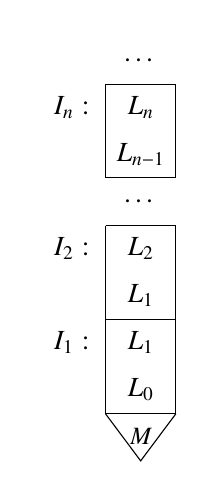
\begin{tikzpicture}
            \matrix (m) [matrix of nodes,nodes={minimum width=2.5em,minimum  height=1.7em}
                        ]
            {
                         & \dots                   \\
                $I_n:$   & $L_n$                   \\
                         & $L_{n-1}$               \\
                         & \dots                   \\
                $I_2:$   & $L_2$                   \\
                         & $L_1$                   \\
                $I_1:$   & $L_1$                   \\
                         & $L_0$                   \\
                         & |[font=\small]|$M$      \\
              };
              \draw (m-1-2.south west) |- (m-4-2.north east) |- (m-1-2.south west);
              \draw (m-4-2.south west) |- (m-6-2.south east) |- (m-4-2.south west);
              \draw (m-4-2.south west) |- (m-8-2.south east) |- (m-6-2.north east);
              \draw (m-8-2.south west) -- (m-9-2.south) -- (m-8-2.south east);
        \end{tikzpicture}
    \caption{A tower of interpreters where each interpreter $I_n$ is written in language $L_{n-1}$ and interprets a language $L_n$, for some $n \geq 0$. In literature the tower often grows downwards, however, in our study we refer to $I_0$ as the base interpreter and grow the tower upwards for convenience. $M$ is the underlying machine (e.g. CPU) on which the base interpreter is executed.}
    \label{fig:tombstone_tower_ex1}
\end{figure}

%First mentions of towers was in 3-LISP. Then Friedman developed a formal account. Black was first to mention collapsing of levels of interpretation. Finally this led to a study specifically focused on towers of interpreters in Pink
%TODO: More detailed explanations (?)
%TODO: switch order of this and next paragraph?

%TODO: bold claim: rephrase
%TODO: Asai MetaOcaml->only with respect to compiled semantics
In the original reflective tower models only minimal attention was given to the imposed cost of performing new interpretation at each level of a tower. Then works by Sturdy \cite{sturdy1993lisp} and Danvy et al.'s language Blond \cite{danvy1988intensions} hinted at the possibility of removing some of this overhead by partially evaluating (i.e., specializing) interpreters with respect to the interpreters below in the tower. Asai et al.'s language \textit{Black} \cite{asai1996duplication} is a reflective language implemented through a reflective tower. The authors use a hand-crafted partial evaluator, and in a later study use MetaOCaml \cite{asai2015compiling}, to efficiently implement the language. Asai and then, using the language Pink \cite{amin2017collapsing}, Amin et al.~demonstrate the ability to compile a reflective language while the semantics of individual interpreters in the underlying tower can be modified. Essentially this is achieved by specializing and executing functions of an interpreter at run-time to remove the cost of multiple interpretation; this effectively \textbf{\textit{collapses}} a tower.
%TODO: verify collapsing methodology + mention clambda (?)

%Parallel to this branch of research towers of interpreters in practice have been encountered in practice at least as long as YACC/LEX exist as Sturdy points out in his analysis of mixed language towers.
Parallel to all the above theoretical research into reflective towers, practical programmers have been working with towers of interpreters to some extent dating back to the idea of language parsers. Writing a parser in an interpreted language already implies two levels of interpretation: %(depicted in figure \ref{fig:tombstone_tower_parser}):
one running the parser and another the parser itself. Other examples include interpreters for embedded domain-specific languages (DSLs) or string matchers embedded in a language both of which form towers of two levels. Advances in virtualization technology has driven increasing interest in software emulation. Viewing emulation as a form of interpretation we can consider interpreters running on virtual hardware, such as the bytecode interpreter in the Java Virtual Machine (JVM) \cite{lindholm2014java}, as towers of interpreters as well.

%\begin{figure}[htp!]
%    \centering
%        \begin{tikzpicture}
%            \matrix (m) [matrix of nodes,nodes={minimum width=3em,minimum  height=1.7em}
%                        ]
%            {
%                String            \\
%                &        Level 1  \\
%                Parser            \\
%                Parser            \\
%                &        Level 0  \\
%                Perl              \\
%                |[font=\small]|M  \\
%              };
%              \draw (m-1-1.north west) |- (m-6-1.south east) |- (m-1-1.north west);
%              \draw (m-3-1.south west) -- (m-3-1.south east);
%              \draw (m-6-1.south west) -- (m-7-1.south) -- (m-6-1.south east);
%        \end{tikzpicture}
%    \caption{Example tower of two levels. Level 0 is a parser interpreted by a Perl interpreter. %The next level is the parser interpreting an input string.}
%    \label{fig:tombstone_tower_parser}
%\end{figure}

However, these two branches of research do not overlap and work on towers of interpreters rarely studied their counterparts in production systems. It is natural to ask the question of what it would take to apply previous techniques in partial evaluation to a practical setting. This is the question Amin et al. pose in their conclusion after describing Pink \cite{amin2017collapsing} and is the starting point for this thesis.

We aim to bring previous work of removing interpretative overhead in towers using partial evaluation into practice. Our study achieves this by constructing a proof-of-concept tower of interpreters that more-closely resembles those in real-world systems. Figure \ref{fig:tombstone} depicts two versions of our experimental tower. Traditionally reflective towers are thought of as completely vertical like the one on the left. However, details such as how a tower grows, shrinks and collapses while executing user programs worked rather mysteriously. We decided to implement our tower using occasional layers of compilation (as shown on the right). The two versions of our tower are extensionally equal since they yield the same output for a given program to evaluate. Part of our study is devoted to evaluating the effect of the intensional structure of towers on the act of collapsing them.

We then collapse the experimental tower under different configurations and evaluate the resulting optimized programs. We demonstrate that given a language capable of expressing types of variables that are available at run-time versus compile-time (i.e., a \textit{multi-level language}) and a type-directed PE (TDPE), a lightweight partial evaluator due to Danvy \cite{danvy1999type} described in section \ref{subsec:tdpe}, we can partially evaluate individual interpreters in a heterogeneous tower and effectively generate code specialized for a user program (hopefully eliminating interpretative overhead in the process). Our work's contributions are:
\begin{enumerate}
	\item Develop an experimental heterogeneous tower of interpreters and a strategy for collapsing it
	\item Evaluate the effect that staging at different levels within our tower has on residual programs
	\item Discuss the effects that heterogeneity in towers imposes on TDPE
	\item Demonstrate issues with and potential approaches to staging abstract machines, specifically a SECD machine, using TDPE
	%TODO: highlight intensional structure of towers and affect on collapsing (move code between layers)
\end{enumerate}

In section \ref{sec:background} we explain background information that covers the fundamental topics we base our experiments and discussions on. We then define \textit{heterogeneity} in towers of interpreters in section \ref{sec:heterogeneity}. In section \ref{sec:recipe} we describe the recipe that the partial evaluation framework Pink \cite{amin2017collapsing} used to construct and collapse meta-circular towers and then show how this recipe changes as a result of heterogeneity. We present the implementation and evaluation of our experimental tower in section \ref{sec:tower}. We systematically describe the process by which we create a heterogeneous tower of interpreters and incrementally collapse it in sections \ref{sec:mslang} through \ref{sec:string_matcher}. We conclude with an evaluation of our findings followed by a discussion of potential future work in section \ref{sec:conclusion}.

\begin{figure}[htp!]
    \centering
    \begin{subfigure}[htp!]{\textwidth}
        \centering
        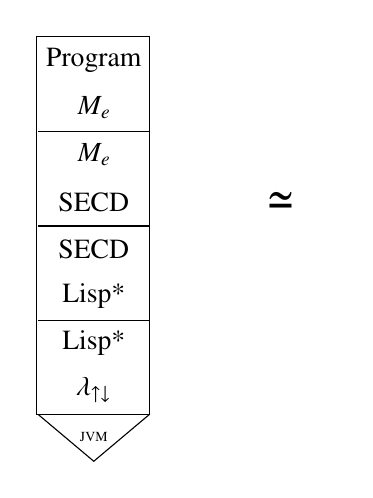
\begin{tikzpicture}
            \matrix (m) [matrix of nodes,nodes={minimum width=4em,minimum  height=1.7em}
                        ]
            {
                Program                 \\
                \mevl                   \\
                \mevl                   \\
                SECD &[6ex] $\boldsymbol{\mathlarger{\mathlarger{\mathlarger{\simeq}}}}$   \\
                SECD                    \\
                Lisp*                   \\
                Lisp*                   \\
                \mslang                 \\
                |[font=\tiny]|JVM       \\
              };
              % With arc
              %\draw (m-1-1.north west) |- (m-8-1.south east) -- (m-1-1.north east);
              %\draw (m-1-1.north east) arc (0:180:0.875);
              
              %Without arc
              \draw (m-1-1.north west) |- (m-8-1.south east) |- (m-1-1.north west);

              \draw (m-2-1.south west) -- (m-2-1.south east);
              \draw (m-4-1.south west) -- (m-4-1.south east);
              \draw (m-6-1.south west) -- (m-6-1.south east);
              \draw (m-8-1.south west) -- (m-9-1.south) -- (m-8-1.south east);
        \end{tikzpicture}%
        \hfill
            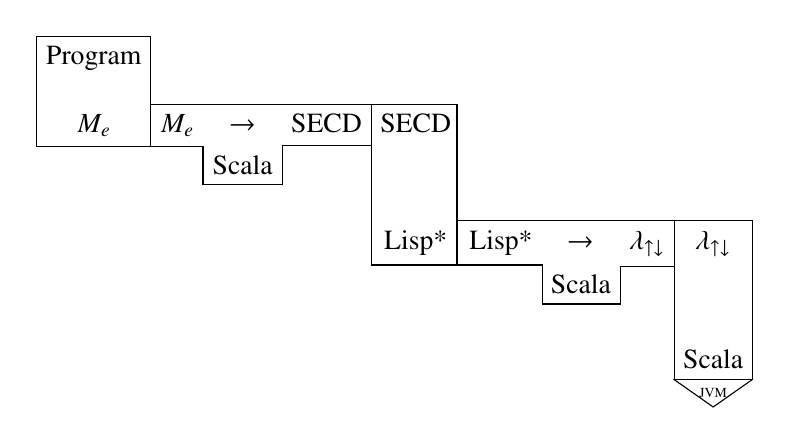
\begin{tikzpicture}
            \matrix (m) [matrix of nodes,%nodes={minimum width=1em,minimum height=1.7em}
                        ]
            {
             Program   &        &       &        &      &                                               \\[2ex]
               \mevl   &  \mevl &  $\to$ &  SECD & SECD &                                               \\
                       &        &  Scala &                                                              \\[3ex]
                       &        &    &       & Lisp* & Lisp* & $\to$ & \mslang & \mslang                \\
                       &        &    &       &      &        & Scala &                                  \\[3ex]
                       &        &    &       &      &        &       &         &  Scala                 \\
                       &        &    &       &      &        &       &         &  |[font=\tiny]|JVM     \\
              };

            % With arc
            %\draw (m-1-1.north west) |- (m-2-2.south west);
            %\draw (m-2-2.south west) -- (m-1-1.north east);
            %\draw (m-1-1.north east) arc (0:180:0.875);

            %Without arc
            \draw (m-1-1.north west) |- (m-2-2.south west) |- (m-1-1.north west);

            \draw (m-2-2.south west) |- (m-2-4.north east) |- (m-3-3.north east) |- (m-3-3.south west) |- (m-2-2.south west);
            \draw (m-2-4.north east) |- (m-4-5.south east) |- (m-2-4.north east);
            \draw (m-4-5.south east) -- (m-4-6.south east) |- (m-5-7.south east) |- (m-4-8.south east) |- (m-6-9.south east)
                    |- (m-4-5.north east);
            \draw (m-4-8.north east) -- (m-4-8.south east);
            \draw (m-6-9.south west) -- (m-7-9.south) -- (m-6-9.south east);
            \end{tikzpicture}
            \caption{Tombstone diagrams that represent two versions of our experimental tower of interpreters. \mevl{} is our toy language described in section \ref{subsec:mevl}, \mslang{} refers to the multi-level language introduced as part of Pink \cite{amin2017collapsing} and Lisp* is \mslang's Lisp based front-end. \textit{JVM} in our diagram also encompasses any underlying machinery necessary to run it. While the left depicts the intuitive view of a tower, we actually implement it using the architecture on the right. Not only is the tower on the right simpler to construct but it also highlights the power of the \textit{lift} operator described in section \ref{subsec:tdpe} and its vital role to collapsing heterogeneous towers.}
            \label{fig:tombstone}
    \end{subfigure}\\[4ex]
    \begin{subfigure}[htp!]{\linewidth}
        \centering
            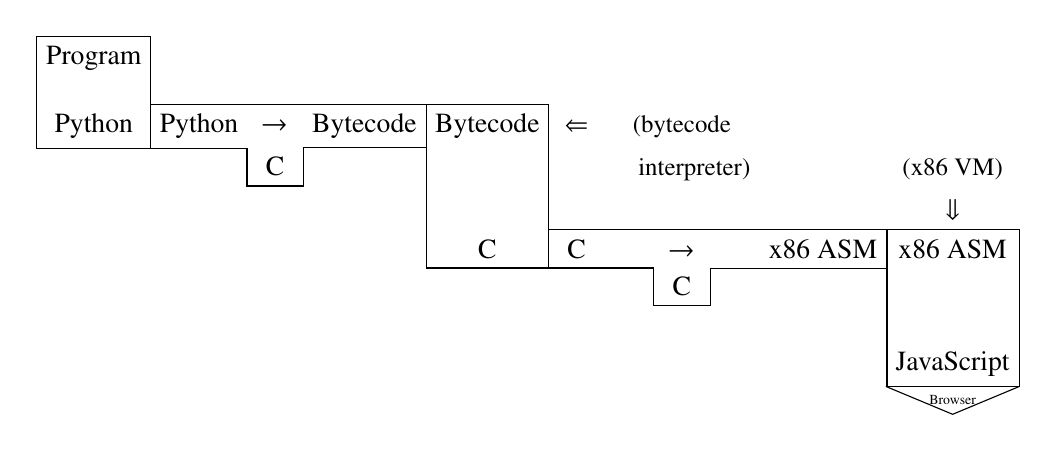
\begin{tikzpicture}
            \matrix (m) [matrix of nodes,nodes={minimum width=2em}
                        ]
            {
             Program    &        &        &           &           &     &       &           &               \\[2ex]
             Python     & Python &  $\to$ &  Bytecode &  Bytecode &   |[font=\small]|$\Leftarrow$  &  |[font=\small]|(bytecode  &           &               \\
                        &        &    C    &           &       &  & |[font=\small]|\quad interpreter) &           &   |[font=\small]|(x86 VM)         \\
                        &        &        &           &           &     &       &           &  |[font=\small]|$\Downarrow$         \\
                        &        &        &           &     C     &   C & $\to$ & x86 ASM   &  x86 ASM      \\
                        &        &        &           &           &     &   C   &           &               \\[3ex]
                        &        &        &           &           &     &       &           &  JavaScript   \\
                        &        &        &           &           &     &       &           &  |[font=\tiny]|Browser      \\
              };

            % With arc
            %\draw (m-1-1.north west) |- (m-2-2.south west);
            %\draw (m-2-2.south west) -- (m-1-1.north east);
            %\draw (m-1-1.north east) arc (0:180:0.73);

            % Without arc
            \draw (m-1-1.north west) |- (m-2-2.south west) |- (m-1-1.north west);

            \draw (m-2-2.south west) |- (m-2-4.north east) |- (m-3-3.north east) |- (m-3-3.south west) |- (m-2-2.south west);
            \draw (m-2-4.north east) |- (m-5-7.south west) |- (m-6-7.south east) |- (m-5-8.south east) |- (m-7-9.south east) |- (m-5-6.north west) |- (m-2-4.north east);
            \draw (m-5-6.north west) -- (m-5-6.south west);
            \draw (m-5-8.north east) -- (m-5-8.south east);
            \draw (m-7-9.south west) -- (m-8-9.south) -- (m-7-9.south east);
            \end{tikzpicture}
            \caption{A hypothetical tower of interpreters that serves as the model for the tower we built (figure \ref{fig:tombstone}). The diagram depicts a JavaScript x86 virtual machine (VM) running a Python \cite{van2011python} interpreter that in turn executes a Python script. In our model, Python is first translated to bytecode which is then interpreted by some bytecode interpreter (written in the C language \cite{kernighan1988c}). \textit{Browser} encompasses the JavaScript interpreter within a browser and any underlying technologies required to host the browser.}
            \label{fig:tombstone_practical}
    \end{subfigure}
    \caption{Comparison between our experimental tower (\ref{fig:tombstone}) and the one we modelled it on  (\ref{fig:tombstone_practical}).}
    \label{fig:tombstone_all}
    %\vspace{-4pt} % Prevent "Float too large" warning
\end{figure}
\newpage

\section{Background}\label{sec:background}
\subsection{\texorpdfstring{$\lambda$}{Lg}-Calculus and de Bruijn Indices}\label{subsec:lambda}
%TODO: debruijn indices visibly used in current project?
Terms in the untyped lambda calculus consist of variables, lambda abstractions and applications of terms. An identifier denotes each variable and determines which lambda binds which variables. Unbound variables are called \textit{free}. Consider now the application of a lambda to a free variable $y$:

\begin{equation*}
    (\lambda x.\lambda y.xy)\:y
\end{equation*}

A $\beta$-reduction of the above term involves an invalid substitution. Replacing occurrences of $x$ with $y$ brings the free variable, $y$, into a scope where a lambda already bound identifier $y$:

\begin{equation*}
    \lambda y.yy
\end{equation*}

Typically one would perform an $\alpha$-conversion (i.e., rename variables) in the lambda appropriately before substitution to prevent a clash of variable names:
\begin{alignat*}{2}
                  & && \: (\lambda y.xy)[x:=y]    \\
    & \equiv_\alpha && \: (\lambda z.xz)[x:=y]    \\
    & \equiv        && \: \lambda z.yz
\end{alignat*}

De Bruijn introduced a canonical lambda notation that prevents such variable name collisions and eliminates the need for $\alpha$-conversions during $\beta$-reductions \cite{de1972lambda}. \textit{De Bruijn indices} denote each variable with an integer that is the number of lambda abstractions between a variable's occurrence and the lambda binding it. Assuming an initial index of $1$ for free variable $y$, the above example in de Bruijn index notation is:
\begin{equation*}
    (\lambda \lambda. 1 \: 0) \: 1
\end{equation*}

Variables and lambdas in \mslang{} (see section \ref{subsec:mslang}) follow the de Bruijn indexing scheme to avoid the complexity of managing variable names and their scopes.

\subsection{Difficulties in Recursion}\label{subsec:recursion}
\textit{Let-expressions} in functional languages are typically syntactic sugar for $\lambda$-abstraction and application. Consider following term:
\begin{equation*}
    (\lambda f.e')(\lambda x.e)
\end{equation*}
As long as $f$ does not occur in $e$ we can rewrite the above in let-expression form:
\begin{minted}[escapeinside=||]{ocaml}
    let f = |$\lambda$|x.e in e'
\end{minted}
%\textit{Let-insertion} is a technique to avoid performing duplicate evaluation of expressions by assigning the result of an expression in a let-statement first

Recursion in programming languages is the ability to reference an expression from within its definition. Permitting the occurrence of $f$ in $e$ in the let-expression above would leave us with a recursive let-expression (also \textit{letrec}). Implementing letrecs is not as straightforward as directly translating from the $\lambda$-calculus and varies between language implementations. Three possible approaches are outlined below.

\subsubsection{Fixed-Point Combinators}
The \textit{fixed point} of function $f$ is some value $x$ such that $f(x)=x$. The function that determines the fixed point of a function is typically labelled \textit{fix} and defined as:
\begin{equation*}
    x = \mathit{fix}(f)
\end{equation*}
By definition of a fixed point we get an equation that resembles recursive function application:
\begin{equation*}
    \mathit{fix}(f) = f (\mathit{fix}(f))
\end{equation*}
The \textit{Y-combinator}, a fixed-point combinator in the lambda calculus, is defined as:
\begin{equation*}
    Y=\lambda f.(\lambda x.f(x x)) (\lambda x.f(x x))
\end{equation*}
This combinator is often used to demonstrate recursion even in languages that do not support it. For some term, $g$, we can write a recursive application as follows:
\begin{equation*}
    Y(g) = g(Y(g))
\end{equation*}
A letrec can now be implemented by using the Y-combinator:
\begin{minted}[escapeinside=||]{ocaml}
    letrec f = Y(|$\lambda f.\lambda x.e$|) in e'
\end{minted}
%TODO: In practice the combinator is less efficient than alternative implementations of recursion...

\subsubsection{Tying the Knot}\label{ssubsec:background_knot}
In languages that permit lazy evaluation or mutation one can create circular data structure definitions using the principle of \textit{tying a knot}. We can create a circular list, \texttt{start}, representing a stream of ones and zeroes as follows \footnote{https://wiki.haskell.org/Tying\_the\_Knot}:
\begin{minted}{haskell}
    let start = 0 : end   in
    let end   = 1 : start in start
\end{minted}
Here, we set (i.e., tie together) the \texttt{end} of the cyclic list to point back to its \texttt{start} and lazy evaluation ensures we do not expand the definition indefinitely.

One can utilize this technique to efficiently implement recursion in a language where recursive definitions are retrieved from some environment upon application. The SECD machine creates a knot in its environment data structure for recursive function application using the \textbf{RAP} instruction (more details in \ref{subsec:secd}) \cite{paulson1995foundations}. For some function (\texttt{f}) SECD creates a closure taking an argument (\texttt{arg}), an expression (\texttt{exp}) and an environment (a list of free-variable values, \texttt{env}) where the first value in the environment is set to the definition of \texttt{f}, \texttt{\&f}:
\begin{minted}[escapeinside=||]{lisp}
    Clo(arg, exp, |\&|f.env)
\end{minted}
Recursive applications of \texttt{f} now reuse its definition repeatedly with only a single definition residing in memory regardless of recursion depth. Despite being more memory efficient, this technique requires mutable data structures or call-by-name semantics, neither of which are supported in \mslang.

\subsubsection{Self-referencing Lambdas}
A final solution is to add self-references to the definition of lambdas. In such a language a lambda named $f$ with argument $x$ and body $e$ is written as: $\lambda_f x.e$. Thus let-expressions and letrecs can simply be expressed as:
\begin{minted}[escapeinside=||]{ocaml}
    let f = |$\lambda_{\_} x.e$| in e'
    letrec f = |$\lambda_{f} x.e$| in e'
\end{minted}
Each lambda implicitly has a reference to itself available for use from within its definition. Pink (section \ref{subsec:mslang}) implements this type of recursion by reserving its first argument for a self-reference.

\subsection{The SECD Machine and Instruction Set (ISA)}\label{subsec:secd}
The SECD machine due to Landin \cite{landin1964mechanical} is a well-studied stack-based abstract machine initially developed in order to provide a model for evaluation of terms in the $\lambda$-calculus. All operations on the original SECD machine are performed on four registers: stack (S), environment (E), control (C), dump (D). \textit{C} holds a list of instructions that should be executed. \textit{E} stores values of free variables (including functions), function arguments and function return values. The \textit{S} register stores results of function-local operations and the \textit{D} register is used to save and restore state in the machine when performing control flow operations. A function we call \textit{step} makes sure the machine progresses by reading next instructions and operands from the remaining entries in the control register and terminates at a \textbf{STOP} or \textbf{WRITEC} instruction, at which point the machine returns all values or a single value from the S-register respectively. As described in section \ref{sec:secd} we add an additional register labelled \textit{F} that holds recursive function definitions for convenience of implementation and partial evaluation.

We now describe the instruction set and implementation details described by Kogge \cite{kogge1990architecture}, which itself is a followup to Henderson's LispKit SECD machine \cite{henderson1980functional}. The three types of SECD instructions are:
\begin{enumerate*}[label=(\arabic*)]
    \item function definition and application
    \item special forms including if-statements
    \item anything else such as arithmetic
\end{enumerate*}. While a table describing all instructions and their transitions is available in figure \ref{fig:secd_kogge}, below we present examples that demonstrate the instructions needed to comprehend later sections.

\subsubsection{Examples}\label{ssubsec:secd_example}

\begin{itemize}
    \item \textbf{LDC} loads an operand (a string or constant) onto the stack (i.e., S-register). Arithmetic instructions such as \textbf{SUB} operate on the top two items of $S$. \textbf{SEL} branches to two different sets of instructions depending on whether the top of \textit{S} is 0 (i.e., false) or not. \textbf{JOIN} jumps back from a branch and resumes the rest of the program while placing the value computed in that branch on top of the stack, e.g.
\begin{minted}[escapeinside=||]{lisp}
    LDC 10 LDC 20 SUB
    LDC 0 GT SEL
        (LDC 5 JOIN)
        (LDC -5 JOIN)
    LDC done
    STOP
    
    |\textcolor{red}{Result: (done -5)}|
\end{minted}
    \item \textbf{LDF} loads a SECD function (i.e., a list of instructions) onto \textit{S}. The argument to the function is the second element in \textit{S}. \textbf{AP} applies the function on top of $S$ to its argument which in the example below is 10. A function can access its argument through the environment register via a lookup using \textbf{LD}. \textbf{RTN} places the value computed in the function onto the stack and returns to the caller.
\begin{minted}[escapeinside=||]{lisp}
    LDC 10 LDF
        (LD (1 1) LDC 20 MPY RTN)
    AP
    STOP

    |\textcolor{red}{Result: (200)}|
\end{minted}

    \item A recursive call consists of two SECD functions: a recursive function and a function that initiates the first recursive call. \textbf{RAP} ties a knot in its environment such that a definition of the closure is accessible during its application; this enables recursion (see section \ref{ssubsec:background_knot}). Additionally, it will initiate the first recursive call. In the below example the recursive function will call itself and increment its argument by 1 and return the argument once it reaches 5. The function finds its definition through \texttt{LD (2 1)} in the environment and subsequently calls itself. For a better understanding of recursive SECD function application see the \textbf{RAP}/\textbf{letrec} analogy in figure \ref{fig:secd_kogge_rap} and the transition table in figure \ref{fig:secd_kogge}.
\begin{minted}[escapeinside=||]{lisp}
DUM NIL LDF
    (LD (1 1) LDC 5 EQ SEL              ;argument == 5?
        (LD (1 1) JOIN)                 ;return argument
        (NIL LDC 1 LD (1 1) ADD         ;increment argument
            CONS LD (2 1) AP JOIN) RTN) ;Recursive call occurs here
CONS LDF
     (NIL LDC 0 CONS LD (1 1) AP RTN) RAP STOP

    |\textcolor{red}{Result: (5)}|
\end{minted}
\end{itemize}

\newpage
\subsection{Interpretation and Compilation}\label{subsec:comp_int}
\begin{figure*}[htp!]
    \centering
    \begin{subfigure}[htp!]{0.4\linewidth}
        \centering
        \begin{picture}(75,75)(0,0)
        \put(0,0){\interpreter{S,L}}
        \end{picture}
        \caption{Interpreter written in language $L$ interpreting a source program in language $S$.}
        \label{fig:tombstone_ex1_int}
    \end{subfigure}%
    \hfill
    \begin{subfigure}[htp!]{0.4\linewidth}
        \centering
        \begin{picture}(75,75)(0,0)
        \put(0,0){\compiler{S,L,T}}
        \end{picture}
        \caption{Compiler written in $L$ that translates from source language $S$ to a target language $T$.}
        \label{fig:tombstone_ex1_comp}
    \end{subfigure}
    \begin{subfigure}{\linewidth}
        \centering
        \begin{picture}(75,75)(0,-35)
        %\put(0,0){\program{P,\compiler{S,\machine[L]{M},\program{P,T}}}}
        \put(0,0){\program{P,\compiler{S,L,\program{P,T}}}}
        \end{picture}
        \caption{Example compilation of a program $P$ from language $S$ to a language $T$}
        \label{fig:tombstone_ex1_prog}
    \end{subfigure}
    \caption{Tombstone diagrams representing interpretation and compilation}
\end{figure*}

%Interpreters vs. compilers
An interpreter reads and directly executes instructions based on an input source program (depicted in figure \ref{fig:tombstone_ex1_int} as a \textit{tombstone diagram} for a pictorial view of composition).
\textit{Definitional interpreters} define the language they implement but not necessarily uniquely \cite{reynolds1972definitional}.

A compiler translates a program into another representation that can subsequently be executed by some underlying machine, or interpreter. A tombstone representation of a compiler is shown in figure \ref{fig:tombstone_ex1_comp}. Here a program $P$ written in language $S$ is compiled to a program $P$ written in $T$; that compiler executes in language $L$. The translation process can occur in a pipeline of an arbitrary number of stages in which a source program is transformed into intermediate representations (IR) to aid its analysis or further transformation.
%TODO: move last sentence(s)
%Modern optimizing compilers consist of stages in which optimization is performed on IR to improve properties of the output code such as execution speed, size or security.

%Just-In-Time (JIT) compilation is the process of compiling or recompiling pieces of a program after execution of it has begun. %The benefit of such on-demand compilation is the ability to make use of a program's execution profiles to make guide optimization %choices. Interpreters for widespread languages such as Python and Julia and frameworks such as GraalVM all make use of JIT %compilation to decrease the cost of interpretation and execute pieces of a program at native speeds. The fact that interpreters %perform compilation as well has blurred the lines between what we can term a compiler as opposed to an interpreter.

In the 1970s Futamura showed that compilers and interpreters are fundamentally related in  an elegant way by three equations also known as the Futamura projections \cite{futamura1999partial}. At its core, the three projections are based on the theory of function \textit{specialization} (or in mathematical terms \textit{projection}). Given a function $f(x,y)$, one can produce a new unique specialized function $f_{x}(y)$ for a fixed value of $x$. In program specialization, we consider $f$ to be a program and the inputs to said program are sets of \textit{static} data $x$ (known before the program's runtime) and \textit{dynamic} data $y$ (only known once a program starts). A \textit{partial evaluator} (also called \textit{residualizer}) is usually denoted by \textit{mix} and takes two inputs: a program and static data to specialize against. Evaluating \textit{mix} (i.e, $\llbracket \mathit{mix} \rrbracket$) against some program $p$ using static data $x$ yields one of possibly many residual programs, $p_x$, for a fixed value of $x$:
\begin{align*}
    p_{x} & = \llbracket mix \rrbracket \:\: (p, x) \\
    out & = \llbracket p_{x} \rrbracket \:\: (y)
\end{align*}
In the above equations $p$ is said to have been \textit{partially evaluated}. Futamura's first projection showed that a compiler for a language $L$, $comp^{L}$, is functionally equivalent to a specializer, $mix$, for an interpreter for language $L$, $int^{L}$. In other words, partially evaluating $int^{L}$ given the source of a L-program, $src^{L}$, achieves compilation:
\begin{align*}
    target & = \llbracket mix \rrbracket \:\: (int^{L}, src^{L}) \\
           & = \llbracket comp^{L} \rrbracket \:\: (src^{L})
\end{align*}
We could now go a step further and instead of specializing an interpreter specialize $mix$ itself and consider the interpreter to be its static input. We pass to $\llbracket \mathit{mix} \rrbracket$ its source, $mix$, and an interpreter, $int^L$; this process is referred to as \textit{self-application}. This yields Futamura's second projection which says that by self-applying a partial evaluator one is able to derive a compiler from an interpreter (i.e., just a semantic description of a language):
\begin{align*}
    comp^{L} = \llbracket mix \rrbracket \:\: (mix, int^{L})
\end{align*}

%TODO: explain "staging transformations"
%Jones MIX rpg. 10: "This is achieved by the automatic splitting of the inter- preter's single binding time into two: compile  time and run time. (This is called a "staging transformation" in Jorring and Scherlis" \cite{jorring1986compilers}
%       \cite{brady2006verified}
In literature a \textit{staging transformation} \cite{jorring1986compilers,brady2006verified}  converts an interpreter into a compiler by splitting the interpreter's direct execution into several stages. The Futamura projections above imply that partial evaluation can be used to introduce two stages to interpretation: one that generates a residual program and another that executes it \cite{jones1993partial}.

A practical realization of the Futamura projections has since been an active area of research. The difficulty in their implementation is the question of how one can best specialize an interpreter and meanwhile also generate the most efficient and correct code; this question is still being explored in the design of partial evaluators to this day \cite{jones1988challenging,jones1993partial}.

\subsection{Type-Directed Partial Evaluation}\label{subsec:tdpe}
%https://link.springer.com/content/pdf/10.1007%2F3-540-47018-2.pdf
%TODO: need to explain dynamic/static twice? it was explained in the previous section already!
Partial evaluation (PE) is a program-optimization technique based on the insight that there is room in programs for statically reducing and producing a specialized (and thus hopefully more efficient) version of itself. The output of a partial evaluator is a \textit{residual program} which, in the ideal case, is a version of the original program where as much computation as possible has been performed with the data that was available at specialization time (i.e., during run-time of the partial evaluator). The portion of data that is known at specialization time is called static and otherwise dynamic. For variables in the program to-be-specialized we refer to its \textit{binding-time} as static if the data it holds during the lifetime of the program is static. Otherwise a variable's binding-time is dynamic.

Partial evaluators generally contain a \textit{binding-time analysis (BTA)} stage which determines whether expressions can be reduced at specialization time or should be preserved in the residual program. A BTA produces a \textit{division} \cite{jones1993partial}; this assigns to each function and variable in a program a binding-time. A division is said to be \textit{congruent} if it assures that every expression that involves dynamic data is marked as dynamic and otherwise as static. A partial evaluator being just an ordinary program, a problem one can run into is non-termination. A congruent division does not always guarantee termination of a PE but when it does we call the division \textit{safe}.
%In our case our division does not ensure termination but rather our implementation and special treatment of function specialization

% EXAMPLE OF CONGRUENCE AND NON-TERMINATION THAT IS APPLICABLE TO STAGED SECD
%Polyvariant binding-time analysis for applicative languages
%http://pages.cs.wisc.edu/~horwitz/CS704-NOTES/9.PARTIAL-EVALUATION.html#div

%There are two types of partial evaluation methodologies :
%\begin{itemize}
%	\item Offline partial evaluation
%	\item Online partial evaluation \cite{cook2011tutorial}
%\end{itemize}

%TODO: Pink really online? TDPE is actually an offline PE technique
In the literature we distinguish between \textit{online} and \textit{offline} partial evaluation \cite{jones1993partial} (or more recently a hybrid between the two due to Shali et al.~\cite{shali2011hybrid}). Offline PE performs a BTA before it begins specialization whereas the online approach makes decisions about whether to residualize expressions once partial evaluation has begun.

%TODO: "A type-directed partial evaluator is thus unconventional in that it does not process the text of a source program, but its compiled (higher-order) value. The normalization effect is not obtained by symbolic interpretation -- it happens en passant in the residualization algorithm" - Pragmatics of type-directed partial evaluation \cite{danvy1996pragmatics}
Danvy devised a method of implementing a partial evaluator solely based on the ideas of normalization in the simply-typed $\lambda$-calculus called \textit{Type-Directed Partial Evaluation} \cite{danvy1999type}. The result is a remarkably simple methodology of implementing residualizers with a binding-time analysis that is completely driven by the \textit{types} of the expressions being specialized. TDPE is built on three core concepts \cite{danvy1997online,grobauer2001second}:
%TODO: well-annotatedness
\begin{tight_enumerate}
    \item BTA produces an expression annotated with static or dynamic binding-times such that reducing static terms yields a \textit{completely dynamic} residual expression (i.e., an expression containing only dynamic variables)
    \item BTA should be able to generate code that includes \textit{binding-time coercions} which are type corrections that help to convert between dynamic and static values for cases where doing so benefits the residualization process
    \item Static reduction (i.e., reduction of expressions annotated as static) is performed by evaluation of an expression and well-formedness of the generated code is guaranteed by the implementing language's type system
\end{tight_enumerate}

TDPE makes use of the type system of a two-level language to direct the residualization of expressions. The output of this lightweight BTA is an expression whose terms are annotated with dynamic or static binding times which when statically reduced yield a purely dynamic expression. Static reduction is performed through regular evaluation of the two-level language's interpreter. TDPE includes a set of operators to convert between dynamic and static terms to aid the optimality of generated code. The two classes of coercion operators are reification (also called \textit{lift}) and reflection both of which are defined on product, function and literal types. \textit{Residualization} is finally defined as performing annotations and binding-time coercions followed by static reduction.

The traditional TDPE \textit{residualize} operation takes as input an expression and a separate object representing the expressions type. Based on the latter argument the residualization algorithm will perform reification according to the rules in figure \ref{fig:tdpe_rules}. As dicussed in section \ref{sec:mslang}, the Pink \cite{amin2017collapsing} partial evaluator implements most of the binding time coercions according to figure \ref{fig:tdpe_rules}'s definitions with the exception of \textit{reflect}, which is implemented using an algorithm attributed to Eijiro Sumii \cite{hatcliff2007partial} to ensure correct order of evaluation of side-effects. The full set of reduction rules are shown in figure \ref{fig:tdpe_rules}.

\subsubsection{Example}
Consider the example \eqref{eq:tdpe_ex1} from Danvy's description of TDPE \cite{danvy1999type}. The aim is to annotate the function applications (denoted by $@$) and definitions with a static (overline) or dynamic (underline) binding-time.
\begin{align}
    \lambda g.\lambda d.(\lambda f.g \:@ \: (f \: @ \: d)\: @ \:f) \: @ \: \lambda a.a \label{eq:tdpe_ex1}
\end{align}

A correct binding-time could be that shown in \eqref{eq:tdpe_ex2a} because after static reduction we obtain \eqref{eq:tdpe_ex2b} which is a completely dynamic expression. However, the duplication of $f$ after reduction and a dynamic redex, $(\underline{\lambda}a.a) \: \underline{@} \: d$, could be optimized away further with a modification to the source expression (i.e., a binding-time coercion). The challenge we are faced with is that $f$ is applied statically but cannot be completely reduced because we also pass it as an argument to a dynamic expression, prohibiting us from residualizing the expression to its fullest.
\begin{figure}[h]
    \begin{align}
        & \underline{\lambda}g.\underline{\lambda} d.(\overline{\lambda} f.g \: \underline{@} \: (f \: \underline{@} \: d) \: \underline{@} \: f) \: \overline{@} \: \underline{\lambda} a.a) \label{eq:tdpe_ex2a} \\
        & \triangleright \:\: \emph{\small{\text{(via static reduction)}}} \nonumber \\
        & \underline{\lambda}g.\underline{\lambda} d.(g \: \underline{@} \: ((\underline{\lambda} a.a) \: \underline{@} \: d) \: \underline{@} \: \underline{\lambda} a.a \label{eq:tdpe_ex2b}
    \end{align}
\end{figure}

We can apply $\eta$-expansion to turn instances of $f$ as a higher-order value into static function applications; TDPE uses this operation during specialization time to increase the number of static expressions it can reduce. The resulting annotations are shown in \eqref{eq:tdpe_ex3a} and the $\eta$-expansion is highlighted in green. After static reduction we obtain the optimal expression in \eqref{eq:tdpe_ex3b} that only contains dynamic values, only a single unfolding of $f$ and no $\beta$-redexes. Danvy then generalizes the $\eta$-expansion into a class of coercions that permit residualization of static values in dynamic contexts, an expression with a dynamic hole \cite{danvy1995essence}. We represent such coercions with a $\downarrow^T$ (or \textit{lift} as we use in later sections) which represents the conversion from a static value of type $T$ to a dynamic value. Using the coercion operator, TDPE would yield the annotation in \eqref{eq:tdpe_ex4}.

\begin{figure}[h]
    \begin{align}
        & \underline{\lambda}g.\underline{\lambda} d.(\overline{\lambda}f.g \: \underline{@} \: (f \: \overline{@} \: d) \: \underline{@} \: \text{\colorbox{green}{$\underline{\lambda} x.f \: \overline{@} x$}}) \: \overline{@} \: \overline{\lambda} a.a \label{eq:tdpe_ex3a} \\
        & \triangleright \:\: \emph{\small{\text{(via static reduction)}}} \nonumber \\
        & \underline{\lambda}g.\underline{\lambda} d.g \: \underline{@} \: d \: \underline{@} \: \underline{\lambda} a.a \label{eq:tdpe_ex3b}
    \end{align}
\end{figure}

\begin{figure}[h]
    \begin{align}
        & \underline{\lambda g}.\underline{\lambda} d.(\overline{\lambda}f.g \: \underline{@} \: (f \: \overline{@} \: d) \: \underline{@} \: \text{\colorbox{green}{(\textit{lift} $f$)}}) \: \overline{@} \: \overline{\lambda} a.a \label{eq:tdpe_ex4} \\
        & \quad \text{where we omit the type parameter on \textit{lift} for simplicity} \nonumber
    \end{align}
\end{figure}

%TODO: revisit reification for recursive functions in TDPE paper
%TODO: lift of recursive functions in Pink
%TODO: Pink also introduces a ``run'' operator

\newpage
\begin{figure}[htp!]
    \centering
    \begin{alignat}{2}
        \text{\underline{\textbf{\emph{Reification (Lifting)}}}}\nonumber \\
        \downarrow^{t} v & = \: && v \\
        \nonumber \\%
        \downarrow^{t_{1} \rightarrow t_{2}} v & = \: && \underline{\lambda} x.\downarrow^{t_{2}}(v\overline{@}(\uparrow_{t_{1}} x)) \\
        & && \quad\text{where $x$ is not a free variable in v} \nonumber \\
        \nonumber \\%
        \downarrow^{t_{1} \times t_{2}} v & = \: && \underline{cons}(\downarrow^{t_{1}} \overline{car} \, v, \downarrow^{t_{2}} \overline{cdr} \, v) \\
        \nonumber \\%
        \mathit{lift} & = \: && \lambda t. \lambda v. \downarrow^{t} v \\
        \nonumber \\%
        %
        \text{\underline{\textbf{\emph{Reflection}}}}\nonumber \\
        \uparrow_{t} e & = \: && e \\
        \nonumber \\%
        \uparrow_{t_{1} \rightarrow t_{2}} e & = \: && \overline{\lambda} v.\uparrow_{t_{2}}(e\underline{@}(\downarrow^{t_{1}} v)) \\
        \nonumber \\%
        \uparrow_{t_{1} \times t_{2}} e & = \: && \overline{cons}(\uparrow_{t_{1}} \underline{car} \, e, \uparrow_{t_{2}} \underline{cdr} \, e) \\
        \nonumber \\%
        \mathit{reflect} & = \: && \lambda t. \lambda e. \uparrow_{t} e
    \end{alignat}
    \caption{Reduction rules for reification (static to dynamic) and reflection (dynamic to static) in TDPE as defined by Danvy \cite{danvy1999type} where $t$ denotes types, $v$ denotes static values, $e$ denotes dynamic expressions. The syntax $cons/car/cdr$ corresponds to the LISP functions of the same name that create a pair, extract the first element of a pair and extract the second element of a pair respectively.}
    \label{fig:tdpe_rules}
\end{figure}
\newpage

%Early partial evaluators, including Jones et al.'s MIX \cite{jones1989mix}, operated exclusively on %untyped languages because it simplified binding time analysis: a single universal type could %represent all static values and would not need to care about whether BTA violated a type-system. To %broaden the applicability of partial evaluation 
%
%* binding time is automatic (or requires annotations only on inputs to program e.g. like in Pink, %which requires knowledege of how the binding-time works. TDPE only requires annotations on base %types from which product, sum and function types' binding-times can be deduced. Pink does not %necessarily have a binding time analysis step which makes it slightly more convenient for manual %annotation)
%* type-directed means we use the type of a term to guide the normalization (i.e. ``extraction %function'' is parameterized by type)
%* TDPE reuses underlying evaluator to perform static evaluation vs code generation. Traditionally %these are performed by the partial evaluator separately in the form of symbolic computation on the %source. Pink takes the former approach
%
%In \cite{danvy1999type} Danvy builts a language in ML that supports and reflection (section 1) and %then shows how partial evaluation of can be achieved using a ``normalization function'':
%%In  summary,  if  one  implements  the  two-level  lambda-calculus  as  in  Sec-tion  1.3, then %reifying  a simply typed,  closed, and completely static  higher-order  function  into  a  dynamic  %expression  automatically  yields  a  representation  of  its  normal form.  In the rest  of this %section,  we illustrate this phenomenon  with  de-compilation,  before  turning to the  %implementation  of  a normalization  function  in  ML.
%
%page 379 explains role of let-insertion
%pg 395: Our framework uses the Eijiro Sumii  approach
%
%page 388: actual description of TDPE
%"We  define  type-directed  partial  evaluation  as normalization  by  evaluation  over  ML values"
%
%page 403: benefits of NbE
%
%jones page. 103: ``The Trick''
%\cite{jones1993partial} page 113: monovariance, polyvariance, congruence in PE, just need to lift products/functions/sum types => reason we stage interpreter that way in Pink and our towers
%Reification according to TDPE (pg. 381): static to dynamic
%Reflection ": dynamic to static
%pg 380: well-annotatedness ensured my Scala's type system (static reduction cannot go wrong guaranteed by evaluation) and the type Exp (result is dynamic if result is Exp=>ensures consequence of annotation turns expression completely dynamic). " Conceptually, well-annotatedness is reduced to ML typeability and static reduction to ML evaluation"
%reflection/reification are forms of binding-time coercions
%pg. 380: "a binding-time coercion maps an expression into a new expression to ensure well-annotatedness between expressions and their contexts during static reduction. In that, binding-time coercions fulfill the same task as, e.g., subtype coercions
%pg. 381: how to coerce a closed, completely static expression into the corresponding dynamic expression. This coercion is achieved using the type-directed translation displayed in Figure 2, which can be seen to operate by "two-level eta expansion"
%
%http://web.cs.ucla.edu/~palsberg/paper/pe99.pdf pg. 2: To obtain consistency, Mix-style partial evaluators [14] coerce static values and contexts to be respectively dynamic values and dynamic contexts, when they encounter a clash. This is acceptable if source programs are first-order and values are either fully static or fully dynamic. However these coercions are excessive for programs with partially static values and contexts.
%http://web.cs.ucla.edu/~palsberg/paper/pe99.pdf and "partial Evaluation of General Parsers": "The Trick"

\subsection{\texorpdfstring{\mslang}{Lg} Overview}\label{subsec:mslang}
%TODO: revisit lift of functions (especially recursive) in Pink
We now provide an overview of the partial evaluation framework developed for Pink \cite{amin2017collapsing} which forms the first two levels of our experimental tower (Lisp* and \mslang{} in figure \ref{fig:tombstone}). At Pink's core is the multi-level language, \mslang{}. The language distinguishes between static values and dynamic values using type constructors \texttt{Val} and \texttt{Exp} respectively. The core evaluator will either residualize, or statically reduce an expression based on the binding-times on its individual terms. The core evaluator (\textit{evalms} in listing~\ref{lst:evalms}) serves as our PE that produces residual programs (i.e., generates code) that are represented by dynamic expressions wrapped in a \texttt{Code} constructor and are in A-normal form \cite{flanagan1993essence}. For example a residualized addition of two literals is,
\mint{scala}|    Code(Plus(Lit(5),Lit(5))))|
%TODO: Eijiro Sumii implementation of TDPE
In \mslang{} the TDPE \textit{reify} operation is called \textit{lift} and converts static \texttt{Val}s into dynamic \texttt{Exp}s. The fact that code generation of expressions can be guided using this single operator, whose semantics closely resemble expression annotation, is attractive for converting interpreters into translators. A user of \mslang{} can stage an interpreter by annotating its source (i.e., wrapping expressions in calls to \mslang{}'s \textit{lift} operator) provided the possibility of changing the interpreter's internals and enough knowledge of its semantics.

%TODO: difference of \mslang to TDPE: dynamic decisions, no type-system required, reflect, Eijiro Sumii, can run dynamic code
%TODO: another difference is that TDPE is automatic on types whereas in Pink the user controls residualization through \textit{manual} annotation of lift
Despite being based on TDPE, the partial evaluation scheme used in Pink is a modified variant which we refer to as \textit{dynamic TDPE}. Firstly, binding time annotations are not performed automatically by the PE but rely on a user annotating the source with \textit{lift}. Secondly, the PE does not require the type of the input expression to be known statically. The ability to dynamically decide on binding-time decisions and not needing a separate type object as input also allows more flexibility in which expressions we want to residualize. The \textit{reflect} operator serves a different purpose to TDPE's specification. Instead of coercing dynamic into static expressions, it adds an expression to the global accumulator of residual terms, \texttt{stBlock}, that is used to generate the specialized code through let-insertion (see line \ref{mline:let_insert} in listing \ref{lst:evalms}). Danvy introduced \textit{let-insertion} into an implementation of TDPE \cite{hatcliff2007partial} to ensure non-idempotent side-effects in expressions duplicated by TDPE are themselves not performed more often than they occur in a source program.

%TODO: 2 levels actually come from statics and dynamic. In literature overlines/underlines indicate stage but in \mslang Val vs Exp determines stage (pg. 379)
\newpage
\begin{longlisting}
    \centering
    \begin{minted}[escapeinside=||,fontsize=\footnotesize]{scala}
// Scala implementation of |\mslang{}|
// expressions (i.e., dynamic data)
abstract class Exp                          // The type of dynamic expressions
case class Lit(n:Int) extends Exp           // Integers
case class Sym(s:String) extends Exp        // Strings
case class Var(n:Int) extends Exp           // Variables (represented as de Bruijn indices)
case class Lam(e:Exp) extends Exp           // Lambdas (no need for argument list due
                                            // to de Bruijn variables)
case class App(e1:Exp, e2:Exp) extends Exp  // Function application
...
// values (i.e., static data)
abstract class Val                          // The type of static expressions
type Env = List[Val]                        // Environment
case class Cst(n:Int) extends Val           // Integers
case class Str(s:String) extends Val        // Strings
case class Clo(env:Env,e:Exp) extends Val   // Closures
case class Code(e:Exp) extends Val          // Residual dynamic data
...

// Converts Expressions (Exp) into Values (Val)
def evalms(env: Env, e: Exp): Val = e match {
    case Lit(n) => Cst(n)
    case Sym(s) => Str(s)
    case Var(n) => env(n)
    case Lam(e) => Clo(env,e)
    case Lift(e) =>
      Code(lift(evalms(env,e)))
    ...
    case If(c,a,b) =>
      evalms(env,c) match {
        case Cst(n) => 
          if (n != 0) evalms(env,a) else evalms(env,b)
        case (Code(c1)) => // Generate an if-statement if conditional is dynamic
          reflectc(If(c1, reifyc(evalms(env,a)), reifyc(evalms(env,b))))
      }
    ...
}
...
var stBlock: List[(Int, Exp)] = Nil
def reify(f: => Exp) = run {
    stBlock = Nil
    val last = f
    (stBlock.map(_._2) foldRight last)(Let) // Let-insertion occurs here |\label{mline:let_insert}|
}
def reflect(s:Exp) = {
    stBlock :+= (stFresh, s)
    fresh()
}
// TDPE-style 'reify' operator (semantics -> syntax)
def lift(v: Val): Exp = v match {
    case Cst(n) => Lit(n)                           // number
    case Str(s) => Sym(s)                           // string
    case Tup(Code(u),Code(v)) => reflect(Cons(u,v)) // pair
    case Code(e) => reflect(Lift(e))                // dynamic expression
    case Clo(env2,e2) =>                            // closure
      stFun collectFirst { case (n,`env2`,`e2`) => n } match {
        case Some(n) =>
          Var(n)
        case None =>
          stFun :+= (stFresh,env2,e2)
          reflect(Lam(reify{ val Code(r) = evalms(env2:+Code(fresh()):+Code(fresh()),e2); r }))
      }
}
...
    \end{minted}
    \caption{Main points of interest of the \mslang{} interpreter written in Scala \cite{odersky2004overview}.}
    \label{lst:evalms}
\end{longlisting}
\newpage

%TODO: do we need below sentence or is front-end mentioned earlier already?
%For convenience the Pink framework additionally provides a LISP front-end that translates LISP s-expressions into \mslang{} expressions.
Pink uses the notion of \textit{stage-polymorphism} introduced by Offenbeck et al. \cite{ofenbeck2017staging} to support two modes of operation:
\begin{enumerate*}[label=(\arabic*)]
	\item ordinary evaluation
	\item generation and subsequent execution of \mslang{} terms
\end{enumerate*}.
Stage-polymorphism allows abstraction over how many stages an evaluation is performed over. This is achieved by operators that are polymorphic over what stage they operate on and is simply implemented as shown in figure \ref{lst:stage_poly_impl}. Whenever the \textit{lift} operator is now used in the \textit{interpreter} or \textit{compiler} it will cause \textit{evalms} to either evaluate or generate code respectively:

\begin{figure}[ht]
\centering
\begin{minted}{lisp}
(let interpreter (let maybe-lift (lambda (x) x) (...)))
(let compiler (let maybe-lift (lambda (x) (lift x)) (...)))
\end{minted}
\caption{``Stage-polymorphism'' implementation from Amin et al.'s Pink \cite{amin2017collapsing}}
\label{lst:stage_poly_impl}
\end{figure}

Now we can combine meta-circular interpreters or compilers in a single invocation of an input program as follows:
\begin{minted}{lisp}
(let int_src       (quote interpreter)
(let comp_src      (quote compiler)
    ((((interpreter int_src) int_src) comp_src) <input quoted program>))))
\end{minted}
The function \textit{quote} is the LISP function that prevents evaluation of its argument. The above example builds a meta-circular tower of three interpreters and a compiler (essentially a staged a interpreter) that run some program (similar to the tower represented in figure \ref{fig:tombstone_collapse_ex_comp}).

%TODO: recipe is actually mentioned in pg. 377 (https://link.springer.com/content/pdf/10.1007%2F3-540-47018-2.pdf)
An advantage of TDPE and why the Pink framework serves as an appropriate candidate PE in our experiments is that it requires no additional dedicated static analysis tools to perform its residualization, keeping complexity at a minimum. Given an interpreter we can stage it by following Amin et al.'s \cite{amin2017collapsing} recipe: lift all terminal values an interpreter returns. Marking returned values as dynamic will dynamize and residualize any operation that includes them.

\subsubsection{Example Staged Interpreter}
The excerpt in figure \ref{fig:pink_source} demonstrates how \textit{lift} annotations are used in staging Pink's interpreter. Any product types (\textit{cons}), function types (\textit{lambda}) and literal types (\textit{num}/\textit{quote}) that are interpreted will be residualized (since they are wrapped in \textit{lift}). In turn any operation on them will also residualize. Effectively we now generate another program that only includes the operations and values of the original expressions (\texttt{exp}) without any interpretative logic. Our interpreter can be said to perform compilation since it generates residual terms in \mslang.
%TODO: mention staging (?)

\begin{figure}[ht!]
\begin{minted}[linenos,escapeinside=||,fontsize=\small]{lisp}
(lambda _ maybe-lift (lambda tie eval (lambda _ exp (lambda _ env
  (if (num?                exp)    |\colorbox{green}{(maybe-lift exp)}|
  (if (sym?                exp)    (env exp)
  (if (sym?           (car exp))
    ...
    (if (eq?  'lambda (car exp))
        |\colorbox{green}{(maybe-lift (lambda}| f x ...
    ...
    |\textcolor{red}{;Meta-circular \textit{lift}}|
    (if (eq?  'lift   (car exp))    (lift ((eval (cadr exp)) env))
    ...
    (if (eq?  'cons   (car exp))
        |\colorbox{green}{(maybe-lift (cons}| ((eval (cadr exp)) env)
                                              ((eval (caddr exp)) env)))
    (if (eq?  'quote  (car exp))   |\colorbox{green}{(maybe-lift (cadr exp))}|
    ...
    ((env (car exp)) ((eval (cadr exp)) env))))))))))))))))))))))))))
  (((eval (car exp)) env) ((eval (cadr exp)) env)))))))))
\end{minted}
\caption{Snippet from Pink's staged interpreter source. Highlighted in green are the polymorphic \textit{lift} expressions we use for binding-time annotations.}
\label{fig:pink_source}
\end{figure}

\section{Heterogeneity}\label{sec:heterogeneity}
%TODO: discuss how side-effects fit into heterogeneity
A central part of our study revolves around the notion of heterogeneous towers. Prior work on towers of interpreters that inspired some these concepts includes Sturdy's work on the Platypus language framework that provided a mixed-language interpreter built from a reflective tower \cite{sturdy1993lisp}, Jones et al.'s Mix partial evaluator \cite{jones1989mix} in which systems consisting of multiple levels of interpreters could be partially evaluated and Amin et al.'s study of collapsing towers of interpreters in which the authors present a technique for turning towers of meta-circular interpreters into one-pass compilers. We continue from where the latter left of, namely the question of how one might achieve the effect of compiling multiple interpreters in heterogeneous settings. We view heterogeneous towers as a generalization of reflective towers and define \textit{heterogeneous} as follows:
\newline
\theoremstyle{definition}
\begin{definition}
	Towers of interpreters are systems of interpreters, $I^L_1, I^L_2, ..., I^L_n$ where $n,k \in \mathbb N_{\ge 1}$ and $I^L_k$ determines an interpreter at level $k$ written in language $L_{k-1}$ and interprets programs in $L_k$.
\end{definition}

%A level here is analogous to an instance of an interpreter within the tower and as such level $n$ implies $I_n$ if not mentioned explicitly otherwise.
\begin{definition}
    \label{def:het}
	Heterogeneous towers of interpreters are towers which exhibit following properties:
	\begin{enumerate}
		\item For any two adjacent interpreters $I_k$ and $I_{k-1}$ where $k \in \mathbb N_{\ge 1}: L_k \not\equiv L_{k-1}$ can hold
		\item For any two adjacent interpreters used in the tower, $I_{k}$ and $I_{k-1}$, the operational semantics and the representation of data can be different between the two
	\end{enumerate}
\end{definition}

\subsection{Absence of: Meta-circularity}
The first generalization described by definition \ref{def:het} is that of mixed languages between levels of a tower. A practical challenge this poses for partial evaluators is the inability to reuse language facilities across interpreters. This also implies that one cannot in general define reflection and reification procedures as in 3-LISP \cite{smith1984reflection}, Brown \cite{wand1988mystery}, Blond \cite{danvy1988intensions}, Black \cite{asai1996duplication} or Pink \cite{amin2017collapsing}.

\subsection{Absence of: Reflection}
Reflection in an interpreter enables the introspection and modification of its state during execution. It is a tool reflective languages can use to embed, for example, debuggers or run-time instrumentation into programs. Reflection in reflective towers implies the ability to modify an interpreter's interpreter which can be beneficial in the implementation of said tools. However, it also allows potentially destructive operations on a running interpreter's semantics which can become difficult to reason about or debug. Towers that we are interested in rarely provide reflective capabilities in every, or even a single, of its interpreters. Thus, we do not support or experiment with reflection in our study.

\subsection{Semantic Gap and Mixed Language Systems}
Danvy et al.~mentioned the possibility of non-reflective non-meta-circular towers early on in his denontational description of the reflective tower model \cite{danvy1988intensions}. The authors explored the idea of having different denotations for data at every level of the tower. However, since it was not the focus of their study, the potential consequences were not further investigated but serve as an inspiration for the second point of definition \ref{def:het}. We call the difference in operational semantics or data representation between two interpreters a \textit{semantic gap}.

Another motivation of ours stems from the realization that systems consisting of several layers of interpretation can feasibly be constructed. A hypothetical tower of interpreters that served as a model for the one we built throughout our work was described in Amin et al.'s paper on collapsing towers \cite{amin2017collapsing} and is depicted as a tombstone diagram in figure \ref{fig:tombstone_practical}. As a comparison our tower is shown in \ref{fig:tombstone}. We replace the x86 emulator with a SECD abstract machine interpreter and Python with our own functional toy language, \mevl. The label \mslang{} represents the multi-level core language from Pink \cite{amin2017collapsing} and Lisp* is the LISP-like front-end to \mslang. Although here the tower grows upwards and to the left, this need not be. The compilers, or \textit{translators}, from \mevl{} to SECD and from Lisp* to \mslang{} have been implemented in Scala purely for simplicity. To realize a completely vertical tower (i.e., consisting of interpreters only), the Lisp*-\mslang{} translator could be omitted such that the \mslang{} interpreter evaluates s-expressions directly. Similarly, the \mevl-SECD compiler could be implemented in SECD instructions itself. However, we argue that the presence of compilation layers in our experimental tower resembles a setting in practice more closely and adds some insightful challenges to our experiments.

\section{General Recipe for Collapsing Towers}\label{sec:recipe}
In this section we describe the methodology that Pink uses to construct and collapse towers and then discuss changes that have to be considered when applying it to a heterogeneous setting.

\subsection{TDPE and Staging a Definitional Interpreter}\label{subsec:stage_def_interp}
Pink defines a multi-level language that differentiates between static and dynamic values. This is essential to express binding-time information. The TDPE-style \textit{lift} (i.e., reify) operator is implemented such that the PE can coerce static to dynamic values.

In his original description of TDPE  Danvy \cite{danvy1999type} showed that we can use above tools to residualize a definitional interpreter with respect to a source program. Pink demonstrates how to stage such an interpreter by wrapping all literal, function and product types in calls to its \textit{lift} operator. Additionally, Pink introduces the concept of \textit{binding-time agnostic staging}. Here, a single interpreter can be used to residualize or simply evaluate a program. In reference to Pink, \textit{staging an interpreter} means lifting types as described above but also activating \textit{code generation mode}, a detail we use in the next section. Code generation mode means an interpreter's polymorphic lift is instantiated such that it invokes \mslang's built-in \textit{lift} (i.e., \textit{compiler} in figure \ref{lst:stage_poly_impl}).

\subsection{Construction and Collapse of a Tower}
\begin{figure}[ht!]
    \centering
    \begin{subfigure}{.4\linewidth}
    \centering
        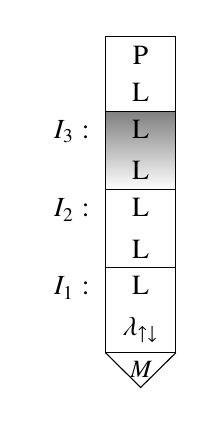
\begin{tikzpicture}
            \matrix (m) [matrix of nodes,nodes={minimum width=2.5em,minimum  height=1.2em}
                        ]
            {
                            &   P                           \\
                            &   L                           \\
             $I_3:$         &   L                           \\
                            &   L                           \\
             $I_2:$         &   L                           \\
                            &   L                           \\
             $I_1:$         &   L                           \\
                            &   \mslang                     \\
                            &   |[font=\small]|$M$          \\
              };
            \draw (m-1-2.north west) |- (m-8-2.south east) |- (m-1-2.north west);
            \draw (m-2-2.south west) -- (m-2-2.south east);
            \draw (m-4-2.south west) -- (m-4-2.south east);
            \draw (m-6-2.south west) -- (m-6-2.south east);
            \draw (m-8-2.south west) -- (m-9-2.south) -- (m-8-2.south east);

            % Background
            \begin{scope}[on background layer]
                \draw[shade] (m-2-2.south west) |- (m-4-2.south east) |- (m-2-2.south west);
            \end{scope}
        \end{tikzpicture}
    \caption{Tower of meta-circular interpreters, $I_k$, in language, $L$, running a program, $P$.}
    \label{fig:tombstone_collapse_ex_int}
    \end{subfigure}%
    \hfill
    \begin{subfigure}{.4\linewidth}
    \centering
    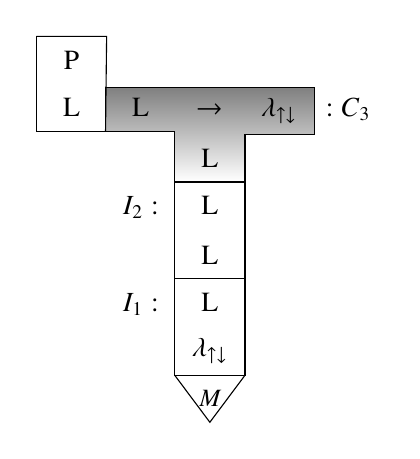
\begin{tikzpicture}
            \matrix (m) [matrix of nodes,nodes={minimum width=2.5em,minimum  height=1.7em}
                        ]
            {
              P     &            &                      &           &           \\
              L     &   L        & $\to$                & \mslang{} &  $:C_3$   \\
                    &            & L                    &           &           \\
                    &   $I_2:$   & L                    &           &           \\
                    &            & L                    &           &           \\
                    &   $I_1:$   & L                    &           &           \\
                    &            & \mslang{}            &           &           \\
                    &            & |[font=\small]|$M$   &           &           \\
             };
            \draw (m-1-1.north west) |- (m-2-1.south east);
            \draw (m-1-1.north west) -- (m-1-1.north east) -- (m-2-2.south west);
            \draw (m-2-2.south west) |- (m-2-4.north east) |- (m-2-3.south east) |- (m-4-3.north west) |- (m-2-2.south west);
            \draw (m-4-3.north west) |- (m-7-3.south east) |- (m-4-3.north west);
            \draw (m-3-3.south west) |- (m-3-3.south east);
            \draw (m-5-3.south west) |- (m-5-3.south east);
            \draw (m-7-3.south west) -- (m-8-3.south) -- (m-7-3.south east);

            % Background
            \begin{scope}[on background layer]
                \draw[shade] (m-2-2.south west) |- (m-2-4.north east) |- (m-2-3.south east) |- (m-4-3.north west) |- (m-2-2.south west);
            \end{scope}
    \end{tikzpicture}
    \caption{Tower whose top interpreter is staged (i.e., converted into a compiler, $C$)}
    \label{fig:tombstone_collapse_ex_comp}
    \end{subfigure}
    \begin{subfigure}{\linewidth}
    \centering
    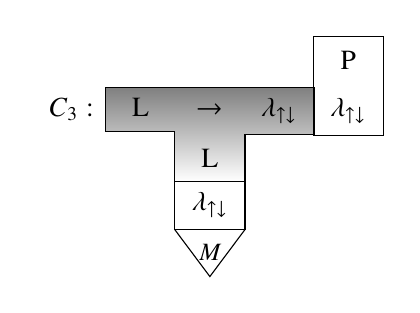
\begin{tikzpicture}
            \matrix (m) [matrix of nodes,nodes={minimum width=2.5em,minimum  height=1.7em}
                        ]
            {
        &     &                       &           &   P       \\
 $C_3:$ & L   & $\to$                 & \mslang   & \mslang   \\
        &     & L                     &           &           \\
        &     & \mslang{}             &           &           \\
        &     & |[font=\small]|$M$    &           &           \\
             };

            \draw (m-1-5.south west) |- (m-1-5.north east) |- (m-2-5.south east) -- (m-2-5.south west) -- (m-1-5.south west);
            \draw (m-2-2.south west) |- (m-2-4.north east) |- (m-2-3.south east) |- (m-4-3.north west) |- (m-2-2.south west);
            \draw (m-4-3.north west) |- (m-4-3.south east) |- (m-4-3.north west);
            \draw (m-4-3.south west) -- (m-5-3.south) -- (m-4-3.south east);

            % Background
            \begin{scope}[on background layer]
                \draw[shade] (m-2-2.south west) |- (m-2-4.north east) |- (m-2-3.south east) |- (m-4-3.north west) |- (m-2-2.south west);
            \end{scope}
    \end{tikzpicture}
    \caption{Final representation of the tower in \ref{fig:tombstone_collapse_ex_int} after collapsing it. All intermediate interpretation (levels $I_1$ to $I_3$) has been eliminated (by evaluating it during PE time) and $P$ has been specialized with respect to the top-most staged interpreter, $C_3$. The residual program $P$ consists of \mslang{} terms in ANF-normal form.}
    \label{fig:tombstone_collapsed}
    \end{subfigure}
    \caption{Tombstones representing the process of collapsing a tower using \mslang{}}
\end{figure}

A tower can then be constructed using a set of meta-circular interpreters each interpreting the next level in the tower. The key benefit of meta-circularity and the basis of collapsing the tower is that the \textit{lift} operator defined in the base evaluator is accessible to each interpreter. We can then stage the user-most interpreter (i.e., the interpreter, $I_n$, running the program provided by the user), as described in section \ref{subsec:mslang}. Although previous work did not provide an insight into the exact effect of staging at different levels in the tower, an intuitive reason we stage at the top-most level is that we want to eliminate as much interpretative overhead as possible which is achieved by collapsing the maximal set of interpreters in the tower. In sections \ref{sec:mslang} to \ref{sec:string_matcher} we provide evidence to support this claim on our experimental tower.

When we now execute the tower (i.e., invoke the partial evaluator at the base) only the top-most evaluator residualizes while all others evaluate. Because of meta-circularity, instead of evaluating a user-value it is now being lifted at all stages essentially propagating binding-time information from top-most interpreter to the base PE. At the last interpreter above the base evaluator, the \textit{lift} now calls the base's actual TDPE-style reify. Effectively after residualization the generated program will only include the values staged at the top-most interpreter while the rest of the tower was reduced at specialization time since it was not evaluated in code-generation mode. Figures \ref{fig:tombstone_collapse_ex_int}-\ref{fig:tombstone_collapsed} depict the above process through tombstone diagrams. We start with a meta-circular tower of interpreters all written in the same language, $L$, and Pink's \mslang{} at the base. After we stage the top-most interpreter (figure \ref{fig:tombstone_collapse_ex_comp}) we can residualize a user program by generating \mslang{} terms; this is essentially the same as removing the intermediate interpreters as they do not get residualized; this yields the collapsed tower in figure \ref{fig:tombstone_collapsed} (assuming the absence of side-effects at individual levels).

\subsection{Effect of Heterogeneity}
\begin{figure}[ht!]
    \centering
        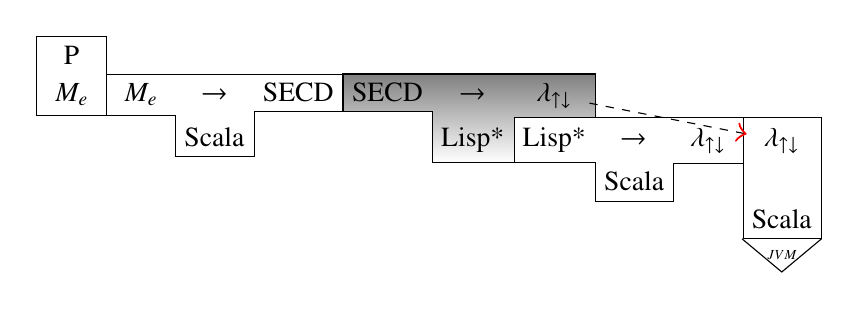
\begin{tikzpicture}
            \matrix (m) [matrix of nodes,nodes={minimum width=2.5em,minimum  height=1.2em}
                        ]
            {
        P       &       &       &       &       &       &         &         &         &                     \\
        \mevl   & \mevl & $\to$ & SECD  & SECD  & $\to$ & \mslang &         &         &                     \\
                &       & Scala &       &       & Lisp* &  Lisp*  & $\to$   & \mslang & \mslang             \\
                &       &       &       &       &       &         & Scala   &         &                     \\
                &       &       &       &       &       &         &         &         & Scala               \\
                &       &       &       &       &       &         &         &         & |[font=\tiny]|$JVM$ \\
            };
            % Outline
            \draw (m-1-1.north west) |- (m-2-2.south east) |- (m-3-3.south east) |- (m-2-5.south east) |- (m-3-7.south east) |- (m-4-8.south east) |- (m-3-9.south east) |- (m-5-10.south east) |- (m-3-7.north east) |- (m-1-1.south east) |- (m-1-1.north west);

            % Dashes
            \draw (m-2-1.north east) -- (m-2-1.south east);
            \draw (m-2-4.north east) -- (m-2-4.south east);
            \draw (m-3-6.south east) |- (m-3-7.north east);
            \draw (m-3-9.north east) -- (m-3-9.south east);

            % Triangle
            \draw (m-5-10.south east) -- (m-6-10.south) -- (m-5-10.south west);
            
            % Background
            \begin{scope}[on background layer]
                \draw[shade] (m-2-5.north west) |- (m-2-5.south east) |- (m-3-6.south east) |- (m-3-7.north east) |- (m-2-5.north west);
            \end{scope}

            % Arrow
            \draw [big arrow] (m-2-7) -- (m-3-10);
        \end{tikzpicture}
    \caption{Our heterogeneous tower of interpreters (\ref{fig:tombstone}) after staging at the SECD level (shaded tombstone). All computation to the left of the staged interpreter is carried into the residual program. The collapse essentially moved the code from above the SECD machine to the base.}
    \label{fig:tombstone_het_collapse_secd}
\end{figure}

\begin{figure}[ht!]
    \centering
        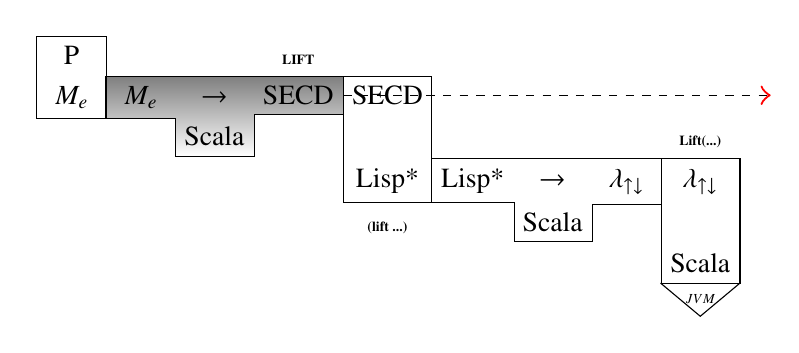
\begin{tikzpicture}
            \matrix (m) [matrix of nodes,nodes={minimum width=2.5em,minimum  height=1.2em}
                        ]
            {
P       &       &       & |[font=\tiny]|\textbf{LIFT}   &                                   &       &         &         &                                   \\
\mevl   & \mevl & $\to$ & SECD                          & SECD                              &       &         &         &                                   \\
        &       & Scala &                               &                                   &       &         &         & |[font=\tiny]|\textbf{Lift(...)}  \\
        &       &       &                               & Lisp*                             & Lisp* & $\to$   & \mslang & \mslang                           \\
        &       &       &                               & |[font=\tiny]|\textbf{(lift ...)}  &       & Scala   &         &                                   \\
        &       &       &                               &                                   &       &         &         & Scala                             \\
        &       &       &                               &                                   &       &         &         & |[font=\tiny]|$JVM$               \\
            };
            % Outline
            \draw (m-1-1.north west) |- (m-2-2.south east) |- (m-3-3.south east) |- (m-2-4.south east) |- (m-4-6.south east) |- (m-5-7.south east) |- (m-4-8.south east) |- (m-6-9.south east) |- (m-4-6.north west) |- (m-2-1.north east) |- (m-1-1.north west);

            % Dashes
            \draw (m-2-1.north east) -- (m-2-1.south east);
            \draw (m-2-4.north east) -- (m-2-4.south east);
            \draw (m-4-6.north west) |- (m-4-6.south west);
            \draw (m-4-8.north east) -- (m-4-8.south east);

            % Triangle
            \draw (m-6-9.south east) -- (m-7-9.south) -- (m-6-9.south west);

            % Background
            \begin{scope}[on background layer]
                \draw[shade] (m-2-2.north west) |- (m-2-2.south east) |- (m-3-3.south east) |- (m-2-4.south east) |- (m-2-2.north west);
            \end{scope}

            % Arrow
            \draw [big arrow] (m-2-4) --++(0:6cm);
        \end{tikzpicture}
    \caption{Our heterogeneous tower of interpreters after staging at the \mevl{} level (shaded tombstone). At each level, starting from \mevl, the \textit{lift} operator is implemented differently but together they achive the effect of moving code from the \mevl{} interpreter to the base.}
    \label{fig:tombstone_het_collapse_mevl}
\end{figure}

We chose the SECD machine to create semantic gaps in our tower through the low-level instruction set that comes with it. For convenience we chose to implement the \mevl{} level as a translator from \mevl{} to SECD instructions instead of writing the interpreter in the instructions directly. Conincidentally, the addition of translation layers into the tower revealed insights into the process of collapsing heterogeneous towers that are not immediately apparent from the composition of tombstones. We describe our observations and further effects of heterogeneity on collapsing towers in the remainder of this section.

While a definitional interpreter can be staged using TDPE by simply lifting values it returns, the process of staging an abstract machine, as we show in section \ref{subsec:secd_staged}, requires careful design of its division rules and consideration of which locations to lift to avoid non-termination at PE-time. Figure \ref{fig:tombstone_het_collapse_secd} depicts the effect of staging the SECD interpreter in our tower. After staging the SECD machine (highlighted in gray) it now operates as a compiler from SECD instructions to \mslang{} terms. Collapsing the tower in this configuration essentially means moving code from the SECD level to the base interpreter across the Lisp* level. Consistent with the composition rules of tombstones, the levels above SECD are residualized and present in the output as well.

In mixed-language towers a \textit{lift} operation is not necessarily available to all interpreters unless explicitly provided at a level. Hence, one approach to propagating binding-time information is to implement a built-in \textit{lift} at all levels below the interpreter that should be staged. As we explain in more detail in section \ref{subsec:secd_staged}, the implementation of \textit{lift} may require us to reverse engineer and transform the representation of closures, pairs or other constructs which the \textit{lift} at the base expects.

%TODO: mention this in contributions (?) and conclusion (?)
A more subtle collapse of our tower occurs when we stage the \mevl{} level (see figure \ref{fig:tombstone_het_collapse_mevl}). In this case staging has a slightly different effect which is not obvious from the tombstones. Since the \mevl{} level is actually a translator already, staging the translator will simply yield another translator. Instead, staging \mevl{} means we generate SECD instructions that \textit{lift} (i.e., signal the PE to residualize) expressions of \mevl{} using a new \textbf{LIFT} instruction (we add it in section \ref{ssubsec:mevl_staged}). As we can see from the annotated tombstone diagram, we use the \textit{lift} operator as a medium to move code through each level to the base where it is residualized. This shows the power of a \textit{lift} construct from a different perspective than previous work on reflective towers. Whereas in reflective towers it worked almost mysteriously to generate new interpreters in a tower \cite{danvy1988intensions}, here we show how it essentially shifts computation down in the tower. Additionally, the larger the shift the less computation has to be residualized.

%tricks involve eta-expansion again

%challenges of staging SECD
%TODO: tower is not framework
%Describe results found: difficulties in heterogeneous setting
%Can be done in multiple ways: can either turn into compiler or let lift sift through
%Describe essence

%TODO: extend using below snippets
%The mix partial evaluation framework \cite{jones1989mix}, Jones et al. demonstrate the PE of a simple interpreter into a language called Mixwell developed by the authors. This is similar in spirit to our framework except it is smaller in height. (section 5 of the paper \cite{jones1989mix}). also mentions removal of layers of meta-interpretation in its conclusion

%Partial Evaluation of Machine Code

%Put together, the three properties imposed by definition \ref{def:het} encourage a generalized solution irregardless of the language or structure of the tower at hand.

\newpage
\section{Construction of an Experimental Heterogeneous Tower}\label{sec:tower}
\subsection{Level 1 \& 2: \texorpdfstring{\mslang}{Lg}}\label{sec:mslang}
%Stage only user-most interpreter (we investigate configurations in this thesis): \textit{wire tower} such that the \textbf{staging commands in $L_{n}$ are interpreted directly in terms of staging commands in $L_{0}$} i.e. staging commands pass through all other layers handing down commands to layers below without performing any staging commands

%In partial evaluation terms, the configurations, i.e. set of run-time computational states, is stored in stBlock while the division, i.e. denotation of static vs dynamic values
The \mslang{} interpreter (running on the JVM) and its Lisp front-end (Lisp* in figure \ref{fig:tombstone}) form the first two levels of the tower, which we mostly keep unchanged from Pink's implementation.

To reduce the amount of generated code we add logic that reduces purely static expressions to \mslang's \textit{reflect}. Reducible expressions include arithmetic and list access operations. We refer to these in later sections as \textit{smart constructors} and they aid in normalizing static expressions that the division (described in section \ref{subsec:secd_staged}) does not permit:

\begin{minted}[escapeinside=||]{scala}
def reflect(s:Exp) = {
    ...
    case _ =>
        s match {
          |\colorbox{green}{case Fst(Cons(a, b)) => a}|
          |\colorbox{green}{case Snd(Cons(a, b)) => b}|
          |\colorbox{green}{case Plus(Lit(a), Lit(b)) => Lit(a + b)}|
          |\colorbox{green}{case Minus(Lit(a), Lit(b)) => Lit(a - b)}|
          |\colorbox{green}{case Times(Lit(a), Lit(b)) => Lit(a * b)}|
          ...
          case _ => // all other cases
            stBlock :+= (stFresh, s)
            fresh()
        }
}
\end{minted}

\subsection{Level 3: SECD}\label{sec:secd}
We chose the SECD abstract machine as one of our levels for following reasons:
\begin{enumerate}
	\item \textbf{Maturity}: SECD was the first abstract machine of its kind developed. Since then it has thoroughly been studied and documented \cite{danvy2004rational,ramsdell1999tail,henderson1980functional} making it a strong foundation to build on.
	\item \textbf{Large Semantic Gap}: A central part of our definition of heterogeneity is that languages that adjacent interpreters interpret are significantly different from each other (see section \ref{sec:heterogeneity}). In the case of SECD's operational semantics, the representation of program constructs such as closures and also the use of stacks to perform all computation deviates from the semantics of \mslang{} and it's LISP front-end and thus satisfies the \textit{semantic gap} property well.
	\item \textbf{Extensibility}: Extensions to the machine, many of which are described by Kogge \cite{kogge1990architecture}, have been developed to support richer features than the ones available in its most basic form including parallel computation, lazy evaluation and call/cc semantics.
\end{enumerate}
An additional benefit of using SECD is that the Pink framework also features a LISP front-end that supports all the list-processing primitives which were used to describe the operational semantics of SECD that we implement (from the small-step semantics and compiler in Kogge's book on symbolic computation \cite{kogge1990architecture}). We model the machine through a case-based evaluator with a \textit{step} function at its core that repeatedly advances the state of the machine until a \textbf{STOP} or \textbf{WRITEC} instruction is encountered.

\subsubsection{Staging a SECD Machine}\label{subsec:secd_staged}
%TODO: essentially these changes:
%   tags for termination
%   lambdas (change representation of functions) for being able to lift in the first place

%https://www.researchgate.net/publication/220989730_Staging_Transformations_for_Abstract_Machines
%Diffs to above: use actual SECD machine, show implementation on the compiler and semantics described in Kogge, approach it from a practical (?) point of view because we need a level with a semantic gap, use partial evaluation instead of pass separation to be able to generate for a different language other than the PE generates, present issues in the process of using TDPE on a stack-based machine, show a general recipe for dealing with non-termination and recursion in SECD-like machine
We design our SECD machine such that it can be staged using Pink's PE; this will enable us to experiment with the effect of staging at different levels of a tower. By definition, a staged evaluator should have a means of generating an intermediate representation, for example residual code, followed by a way to execute it (directly or through further stages). Partial evaluation allows us to split the SECD interpreter's execution into two stages:
\begin{enumerate*}[label=(\arabic*)]
    \item reduce static values and residualize dynamic values
    \item execute the residual expressions
\end{enumerate*}.
%previous work->used pass separation to generate interpreters for a dynamically generated %abstract machine language
%our work->use partial evaluation on a SECD machine whose implementation provides the necessary %properties for partial evaluation to work correctly and efficiently; less intrusive; given the %stack and can't chose the levels beneath or above

From the architecture of a SECD machine the intended place for free variables and user input to live in is the environment register. For example an expression as the following uses a free-variable, $y$, which is unknown and a residualizer would classify as dynamic:

\mint{lisp}|    ((lambda (x) (x + y)) 10)|
This translates to following SECD instructions:

\mint{lisp}|   NIL LDC 10 CONS LDF (LD (1 1) LD (2 1) ADD RTN) AP STOP|

We load only a single value of 10 into the environment and omit the second argument that \textbf{LDF} expects and uses inside its body. Instead \textbf{LDF} simply loads at a location not yet available (i.e., \mbox{\texttt{LD (2 1)}}) and trusts the user to provide the missing value at run-time.

Prior to deciding on the methodology for code generation we need to outline what stages one can add to the evaluation of the SECD machine and how the binding-time division is chosen. We define our division by where static values can be transferred from. If a dynamic value can be transferred from a register, $A$, to another register, $B$, we classify register $B$ as dynamic. We define the binding-time of a SECD register to be the combination of all possible binding-times of elements of a register. When a register can hold both dynamic and static values, the register's binding time is referred to as \textit{mixed}. The full division for each SECD register is provided in table \ref{tbl:secd_division}.

\begin{table}[!htbp]
  \centering
  \begin{tabular}{|p{3cm}|p{3cm}|p{6cm}|}
 	\hline
 	\thead{SECD Register}	&	\thead{Classification}	&	\thead{Reason}	\\ \hline
	$S$ (Stack)				&	\vtop{\hbox{\strut Mixed}\hbox{\strut (mostly dynamic)}}				&	Function arguments and return values operate on the stack \textit{and} dynamic environment and thus are mostly dynamic. Elements of the stack can, however, be static in the case of thunks described in section \ref{ssubsec:knot} \\ \hline

	$E$ (Environment)		&	\vtop{\hbox{\strut Mixed}\hbox{\strut (mostly dynamic)}}	&	 Most elements in this register are dynamic because they are passed from the user or represent values transferred from the stack. Since the stack can transfer static values on occasion the environment can contain static values as well. \\ \hline

	$C$ (Control)				&	Static				& We make sure the register only receives static values and is thus static (we ensure this through eta-expansion in section \ref{subsec:secd_staged})  \\ \hline

	$D$ (Dump)				&	Mixed				&	Used for saving state of any other register and thus elements can be both dynamic, static or a combination of both \\ \hline

	$F$ (Functions)		&	Static				&	Since it resembles a \textit{control} register just for recursively called instructions we also classify it as static \\

	\hline
  \end{tabular}
  \caption{Division rules for our approach to staging a SECD machine}
  \label{tbl:secd_division}
\end{table}

We refer to our division as coarse grained since dynamic values pollute whole registers that could serve as either completely static or mixed valued. An example would be a machine that simply performs arithmetic on two integers and returns the result. The state machine transitions would occur as shown in table \ref{tbl:secd_example1}. As the programmer we know there is no unknown input and the expression can simply be reduced to the value ``30'' following the SECD small-step semantics. However, by default our division assumes the S-register to be dynamic and thus generates code for adding two constants. In such cases the smart constructors discussed in section \ref{sec:mslang} allow as to reduce constant expressions that a conservative division would otherwise not. We keep this division as the basis for our staged SECD machine since it is less intrusive to its interpreter and still allows us to residualize efficiently.

Through its LISP front-end the \mslang{} evaluator can operate as a partial evaluator by exposing its \textit{lift} operator. We stage our SECD machine interpreter by annotating its source with said \textit{lift} according to the division in table \ref{tbl:secd_division}.

\begin{table}[htp!]
\centering
\begin{tabular}{|c|c|}
\hline
\thead{Step}	&	\thead{Register Contents}	 \\ \hline
\multicolumn{1}{|l|}{0}                     & \multicolumn{1}{l|}{\begin{tabular}[c]{@{}l@{}}s: ()\\ e: ()\\ c: (LDC 10 LDC 20 ADD WRITEC)\\ d: ()\end{tabular}} \\ \hline
\multicolumn{1}{|l|}{1}                     & \multicolumn{1}{l|}{\begin{tabular}[c]{@{}l@{}}s: (10) \\ e: () \\ c: (LDC 20 ADD WRITEC) \\ d: ()\end{tabular}}   \\ \hline
\multicolumn{1}{|l|}{2}                     & \multicolumn{1}{l|}{\begin{tabular}[c]{@{}l@{}}s: (20 10) \\ e: () \\ c: (ADD WRITEC) \\ d: ()\end{tabular}}       \\ \hline
\multicolumn{1}{|l|}{3}                     & \multicolumn{1}{l|}{\begin{tabular}[c]{@{}l@{}}s: (30) \\ e: () \\ c: (WRITEC) \\ d: ()\end{tabular}}              \\ \hline
\multicolumn{1}{|l|}{4}                     & \multicolumn{1}{l|}{\begin{tabular}[c]{@{}l@{}}s: () \\ e: () \\ c: () \\ d: ()\end{tabular}}
\\ \hline
\multicolumn{2}{|l|}{\begin{tabular}[c]{@{}l@{}}Generated Code (without smart constructor):\\ \quad(lambda f0 x1 (+ 20 10)) \end{tabular}} \\ \hline
\multicolumn{2}{|l|}{\begin{tabular}[c]{@{}l@{}}Generated Code (with smart constructor):\\ \quad(lambda f0 x1 30)\end{tabular}}
\\ \hline
\end{tabular}
\caption{Example of SECD evaluation and \mslang code generated using our PE framework. The division follows that of table \ref{tbl:secd_division}.}
\label{tbl:secd_example1}
\end{table}

%"The main semantic challenge is that we want to implement a definitional interpreter for SECD in Pink, so we need big-step instead of small-step like in Fig 7.12 of Kogge, and we need to use the underlying recursive lambda of Pink instead of mutation for letrec." - Nada

\newpage
\subsubsection{The Interpreter}\label{subsec:secd_interp}
\begin{figure}[htp!]
\centering
\begin{minted}[fontsize=\small,escapeinside=||,linenos]{lisp}
(let SECDMachine (lambda _ stack (lambda _ dump (lambda _ control (lambda _ environment
    (if (eq? 'LDC (car control))
        (((((SECDMachine (cons (cadr control) stack)) dump) (cdr control)) environment)
    (if (eq? 'DUM (car control))
        (((((SECDMachine stack) dump) (cdr control)) (cons '() environment))
    (if (eq? 'WRITEC (car control))
        (car s)
    ...
    ...)))))))
    (let initStack '()
    (let initDump '()
        (lambda _ control (((((SECDMachine initStack) initDump) control)))) |\label{mline:machine_init}|
\end{minted}
\caption{Structure of interpreter for SECD machine (unstaged). Lambdas take two arguments, a self-reference for recursion (which is ignored through a ``\_'' sentinel) and a caller supplied argument. All of SECD's stack registers are represented as LISP lists and initialized to empty lists. ``...'' indicate omitted implementation details}
\label{lst:secd_unstaged}
\end{figure}

Our staged machine is written in \mslang's LISP front-end as a traditional case-based interpreter that dispatches on SECD instructions stored in the C-register. The structure of our SECD interpreter, \textit{SECDMachine}, without annotations to stage it is shown in figure \ref{lst:secd_unstaged}. Of note are the single-argument self-referential lambdas and the out-of-order argument list to the machine. To allow a user to supply instructions to the machine we return a lambda that accepts input to the control register ($C$) in line \ref{mline:machine_init}. Once a SECD program is provided we curry \textit{SECDMachine} with respect to the \textit{environment} which is where user-supplied arguments go. An example invocation is \mint{lisp}|  ((SECDMachine '(LDC 10 LDC 20 ADD WRITEC)) '())| where the arguments to the machine are the arithmetic example of table \ref{tbl:secd_example1} and an empty environment respectively.

To stage our interpreter we annotate terms that we want to be able to generate code for with the stage-polymorphic \textit{maybe-lift} operators (defined in figure \ref{lst:stage_poly_impl}). With our division in place (see table \ref{tbl:secd_division}) we simply wrap in calls to \textit{maybe-lift} all constants that potentially interact with dynamic values and all expressions that add elements to the stack, environment or dump. Figure \ref{lst:secd_staged1} shows these preliminary annotations. We wrap the initializing call to the SECD machine in \textit{maybe-lift} (line \ref{mline:lift_machine}) as well because we want to specialize the machine without the dynamic input of the environment provided yet.

\begin{figure}[ht]
\centering
\begin{minted}[escapeinside=||,linenos,fontsize=\footnotesize]{lisp}
(let SECDMachine (lambda _ stack (lambda _ dump (lambda _ control (lambda _ environment
    (if (eq? 'LDC (car control))
        (((((SECDMachine (cons |\colorbox{green}{(maybe-lift }|(cadr control)|\colorbox{green}{)}| stack)) dump) (cdr control)) environment)
    (if (eq? 'DUM (car control))
        (((((SECDMachine stack) dump) (cdr control)) (cons |\colorbox{green}{(maybe-lift }|'()|\colorbox{green}{)}| environment))
    (if (eq? 'WRITEC (car control))
        (car s)
    ...
    ...)))))))
    (let initStack '()
    (let initDump '()
        (lambda _ ops |\colorbox{green}{(maybe-lift }|(((SECDMachine initStack) initDump) ops))|\colorbox{green}{)}|))))) |\label{mline:lift_machine}|
\end{minted}
\caption{Annotated version of the SECD interpreter in figure \ref{lst:secd_unstaged} with differences highlighted in green. The function \textit{maybe-lift} is used to signal to the PE that we want to generate code for the wrapped expression. Here we follow the division of table \ref{tbl:secd_division}.}
\label{lst:secd_staged1}
\end{figure}

%TODO: reword
This recipe is not enough, however, because of the conflicting nature of our SECD machine's stepwise evaluation with TDPE's static reduction by evaluation. To progress in partially evaluating the machine we must take state-transition steps and essentially execute it at PE time. A consequence of this is that the PE can get into a situation where dynamic values are evaluated in static contexts potentially leading to undesired behaviour such as non-termination at specialization time (see \ref{ssubsec:knot} for more details). Where we encountered this particularly often is the accidental lifting of SECD instructions or specialization of recursive SECD function calls.

Key to us removing interpretative overhead of the SECD machine is the elimination of its unnecessary instruction dispatch logic from the specialized code, whose effect on interpreter efficiency was studied extensively by Ertl et al. \cite{ertl2003structure}. Since the SECD program is known at PE time and thus has static binding time, we do not want to lift the constants against which we compare the control register. However, if we put something into the control register that is dynamic we are suddenly comparing dynamic and static values which is a specialization time error at best and non-termination of the PE at worst.

%TODO more accurate explanation of RAP and specifically how it forms the environment loop
Another issue we dealt with in the process of writing the staged SECD interpreter is the implementation of the \textbf{RAP} instruction which is responsible for recursive applications. The instruction essentially works in two steps. First the user creates two closures on the stack. One which holds the recursive function definition and another which contains a function that initiates the recursive call and prepares any necessary arguments. \textbf{RAP} calls the latter and performs the subtle but crucial next step. It forms a knot in the environment such that when the recursive function looks up the first argument in the environment it finds the recursive closure. According to Kogge's \cite{kogge1990architecture} description of the SECD operational semantics this requires an instruction that is able to mutate variables. Given the choice between adding support for an underlying \texttt{set-car!} instruction in \mslang{} or extending the SECD machine such that recursive function applications do not require mutation in the underlying language we decided to experiment on the latter.
%TODO: bring back set-car! methodology later if needed

%An issue that became apparent during the conversion from a regular to a staged SECD machine is the machine's stepwise operational semantics proneness to non-termination when applying our NBE-style partial evaluation. This is particularly prominent whenever an if-statement decides the arguments to the next step of the machine.

%Resort to online partial evaluation at certain points not because it helps optimize more aggressively, as that is usually the reason to use online PE, but rather to avoid non-termination in our model.

%the latter because it was simpler to add such extension than rewriting the Pink framework and would show additional use cases for \mslang. For a thorough treatment of side-effects in partial evaluators we defer to previous work by Asai et al. who develop a partial evaluator for an imperative $\lambda$-calculus with support for mutating cons-cells and imperative LISP features.

%Putting the above solutions together yields the new staged interpreter in figure FIGURE.

%Difficulties arise whenever we attempt to mix dynamic and static values since its easy to want to compare and operate on the stack. Thus we need another register that is purely reserved for static values. To keep the amount of noise in the generated code lower one also needs to be careful to only mix static values into dynamic registers when necessary (show example of SECD noisy instrs in the generated code e.g. in simple non-recursive curried lambda or matcher code pre-noise reduction vs. factorial generated code).

%If we are willing to diverge further from the SECD instruction set we can implement recursive function application by omitting the \textit{fns} register, modifying LDF to wrap SECD instruction in a lambda as before but remove the RAP and DUM instructions all-together leaving it up to LD and AP to locate and apply the recursive lambda. Essentially what this resembles is the eta-expansion technique to guarding higher-order static data from dynamic contexts typically used in TDPE \cite{danvy1995essence}. The small-step semantics of this approach are as follows:

%TODO: explain what tying a knot means tying knot in data instead of in code
\subsubsection{Tying the Knot}\label{ssubsec:knot}
We now provide a substantial redesign to the internal \texttt{RAP} calling convention. Without the ability to tie a knot in the environment we need a different way of achieving recursion in SECD. Additionally we need to design the internals of the machine such that we can stage it using Pink's TDPE.

Following example, in which a recursive function decrements a user provided number down to zero, demonstrates the issue of partially evaluating a recursive call in using SECD small-step semantics:

\begin{figure}
\centering
\begin{minted}[escapeinside=||,linenos,fontsize=\footnotesize]{lisp}
DUM NIL LDF ;|\small{Definition of recursive function starts here}\label{mline:rec_ex1_rec_fn}|
    (LD (1 1)
     LDC 0 EQ ;|\small{counter == 0?}\label{mline:rec_ex1_base_chk}|
     SEL
       (LDC done STOP) ;|\small{Base case: Push "done" and halt}\label{mline:rec_ex1_base_exit}|
       (NIL LDC 1 LD (1 1) SUB CONS LD (2 1) AP JOIN) ;|\small{Recursive Case: Decrement counter}|
     RTN)
    CONS LDF
    (NIL LD (3 1) CONS LD (2 1) AP RTN) ;|\small{Set up initial recursive call}\label{mline:rec_ex1_setup_fn}|
    RAP
\end{minted}
\caption{Example recursive function application}
\label{lst:secd_recursion_ex1}
\end{figure}

Our PE would not terminate were we to specialize this program by simply evaluating the machine. The exit out of the recursive function (defined on line \ref{mline:rec_ex1_rec_fn}) occurs on line \ref{mline:rec_ex1_base_exit} but is guarded by a conditional check on line \ref{mline:rec_ex1_base_chk}. This conditional compares a dynamic value (i.e., \mbox{\texttt{LD (1 1)}}) with a \mbox{constant 0}. By virtue of our division's congruence the \mbox{0-literal} and whole if-statement are classified as dynamic. However, for TDPE this dynamic check does not terminate the PE but instead attempts to reduce both branches of the statement. Since both branches are simply a recursive call of the \textit{step} function we hit this choice again repeatedly without terminating because we have no way of signalling to stop partially evaluating.
\newpage
Following example highlights this in the internals of the machine:
\begin{listing}
    \begin{minted}[escapeinside=||,linenos,fontsize=\footnotesize]{lisp}
(if (eq? 'SEL (car control))
  |\colorbox{green}{(if (car stack)}| ;Do not know the result because value on stack is dynamic
    ;Make another step in machine. Will eventually hit this condition again
    ;because we are evaluating a recursive program
    (((((|\colorbox{green}{machine}| (cdr stack)) (cons (cdddr control) dump)) fns) (cadr control)) environment)
    (((((machine (cdr stack)) (cons (cdddr control) dump)) fns) (caddr control)) environment))
    \end{minted}
\end{listing}

Highlighted are the locations at which our partial evaluator does not terminate. TDPE attempts to evaluate both branches because we cannot determine the outcome of the conditional.

Instead of evaluating the recursive call, we want to instead generate the function definition and call in our residual program. What we now need to solve is how one can produce residual code for these SECD instructions that are ``to be-called-recursively''. The key to our approach is to reuse \mslang's ability to lift closures. Figure \ref{fig:secd_semantics_noset} shows the modifications to the operational semantics of Kogge's SECD description \cite{kogge1990architecture} which allow it to be partially evaluatable with a TDPE and do not require a \texttt{set-car!} in the underlying language. The idea is to wrap the recursive SECD instructions in a closure at the LISP-level and use Pink lambda's ability to self-reference to achieve recursion. Closures also allow us to produce residual code for SECD functions, which previously was not possible since they were simply represented as lists of instructions.

Before explaining our modifications to the SECD instruction set in detail we briefly outline three significant changes to note:
\begin{enumerate}
    \item SECD functions are now lambdas that wrap a call to the implicit state transition which is our way of achieving recursion without tying a knot. This also helps our aim of staging the machine since Pink's \textit{lift} operates on lambdas and allows us to residualize entire function bodies.
    \item The \textbf{RTN} instruction aids termination of TDPE by preventing it to evaluate the machine (i.e., perform state transitions) further upon detection of appropriate tags in \textit{D}. This ensures that we can terminate the unfolding of recursive calls.
    \item Instructions \textbf{AP}/\textbf{RTN}/\textbf{LIFT} all feature calls to a \textit{lift} operator that follow the division established earlier in table \ref{tbl:secd_division} to stage the SECD interpreter
\end{enumerate}

\begingroup
\allowdisplaybreaks
\begin{figure}[htp!]
\centering
\begin{alignat}{5}
		\text{s e (} \mathbf{LDF} \text{ ops.c) d f} & \longrightarrow \: && \text{(($\lambda$e{\ts}.(run@({\ts}() e{\ts} ops {\ts}ret f))) ops.e).s e c d f} \label{eq:secd_sem_ldf} \\
		\nonumber \\%
		%
		\text{(entryClo recClo.s) e (} \mathbf{RAP}\text{.c) d f} & \longrightarrow \: && \text{{\ts}() e entryOps (s e c f.d) (lift@rec (mem.recEnv)).f} \label{eq:secd_sem_rap} \\
		\text{where (entryFn (entryOps entryEnv))} & := && \text{entryClo} \nonumber \\
		\text{(recFn (recOps recEnv))} & := && \text{recClo} \nonumber \\
		\text{rec} & := && \text{$\lambda$env.(run@({\ts}() env recOps {\ts}ret (rec (mem.recEnv)).f))} \nonumber \\
		\text{mem} & := && \text{((s e c f.d) (recOps.recEnv).f)} \nonumber \\
		\nonumber \\%
		%
		\text{s e (} \mathbf{LDR} \text{ (i j).c) d f} & \longrightarrow \: && \text{(locate@(i j f)).s e c {\ts}ldr.d f} \\
		\nonumber \\%
		%
		\text{v.s e (} \mathbf{RTN}\text{.c) (s{\ts} e{\ts} c{\ts}  d{\ts}  f{\ts}.d) f} & \longrightarrow \:
		 && \text{lift@v} \qquad\quad\:\text{\textit{if d-register is tagged with {\ts}ret}}	\\
		 & && \text{$\lambda$x.(fn@(lift@(x.env)))} \nonumber \\
		 & && \qquad\text{where (fn (ops env))} := \text{v} \nonumber \\
		 & && \qquad\qquad\qquad\text{\textit{if d-register is tagged with {\ts}ldr}} \nonumber \\
 		 & && \text{(v.s{\ts})  e{\ts}  c{\ts}  d{\ts}  f{\ts}}	\:\:\:\text{\textit{otherwise}} \nonumber \\
 		\nonumber \\%
 		%
		\text{s{\ts} e (} \mathbf{AP}\text{.c) env{\ts} f} & \longrightarrow \: && \text{(fn@(lift@(x.env))).s e c d f} \\
		& && \quad\text{where ((fn (ops.env)) x.s)} := \text{s{\ts}} \nonumber \\
		\nonumber \\%
		%
		\text{(v.s) e (} \mathbf{LIFT}\text{.c) d f} & \longrightarrow \: \label{eq:secd_sem_lift}
		 && \text{res.s e c d f}   \\
		 \text{where res} & := && \text{lift@v\quad \textit{if (num? v) or (sym? v)}} \nonumber \\
		 & && \text{lift@($\lambda$x.(run@({\ts}() x.env ops {\ts}ret f)))} \quad\text{\textit{if (clo? v)}} \nonumber \\
		 & && \quad \text{where (fn (ops env))}:= \text{v} \nonumber
\end{alignat}
\caption{Modifications to the SECD operational semantics by Kogge \cite{kogge1990architecture}. The original transitions are shown in figure \ref{fig:secd_kogge}. The function \textit{run} takes state-transition steps according to \textit{C} until the machine halts. The function \textit{locate} returns an element at index (i,j) from a multi-dimensional list. An ``@'' denotes function application and registers \textit{S, E, C, D, F} are represented by \textit{s, e, c, d, f} respectively. The syntax \textit{num?/sym?/clo?} are conditions satisfied when their argument is a number, string or a closure respectively.}
\label{fig:secd_semantics_noset}
\end{figure}
\endgroup
\newpage

%TODO essence of new semantics
Firstly, equation \ref{eq:secd_sem_ldf} augments the representation of functions in the SECD machine (simply lists of instructions) with a thunk that accepts an environment and upon invocation runs the abstract machine with the instructions put into the C-register by \textbf{LDF}. Working with thunks makes the necessary changes to stage the machine less intrusive and effectively prevents the elements of the control register being marked as dynamic; this means we can safely lift all elements in \textit{S} when we try following our division. This is in line with the ideas of Danvy et al. \cite{danvy1995essence} which showed that eta-expansion can enable partial evaluation by hiding dynamic values from static contexts.

Note also that we add a new functions register, which we refer to as the \textbf{F-register}\footnote{In his description of the SECD machine Kogge \cite{kogge1990architecture} uses \textit{F} to label the register that holds a list of free memory locations in the machine. We do not require such register in our implementation and thus repurpose it to store recursive function definitions}, that is responsible for holding our closures that wrap recursive instructions of a \textbf{RAP} call. In the traditional SECD machine both the recursive and the calling function are kept in the environment, loaded onto the stack using \textbf{LD} and subsequently called using \textbf{AP}. However, for simplicity we keep recursive functions in \textit{F} to distinguish them from free variables in \textit{E} and aid debuggability. Thus we introduce a new \textbf{LDR} instruction that returns the contents of the F-register by index, just as \textbf{LD} does for the E-register.
%TODO: debuggability enough justification for separate register?

Modification to the \textbf{RAP} instruction are described by \eqref{eq:secd_sem_rap}. As in the original semantics it still expects two closures on top of the stack: one that performs the initial recursive call which we refer to as \textit{entryClo} and another that represents the actual set of instructions that get called recursively, \textit{recClo}. Each closure consists of a function (\textit{entryFn} or \textit{recFn}), the SECD instructions these functions execute (\textit{entryOps} or \textit{recOps}) and an environment (\textit{entryEnv} or \textit{recEnv}). \textbf{RAP} then lifts and appends a newly constructed recursive closure to \textit{F}. The \textit{lift} is necessary because we want the definition of the recursive function to appear in the residual program. The new closure when applied to an environment, runs the machine with the \textit{C} containing instructions of the recursive function body. Additionally, applying the closure places a \textit{{\ts}ret} tag onto the \textit{D} which is later used as an indicator to stop evaluating the current call; this is crucial to aid termination during specialization time.

In the original semantics of SECD, \textbf{RTN} would restore the state of all registers from the dump and add the top most value of the current S-register back onto the restored S-register. This modelled the return from a function application. As we showed earlier in this section, taking another step in the machine when specializing a recursive function will lead to non-termination of our specializer. Thus, we simply stop evaluation when returning from a function by chgecking \textit{D} for a \textit{{\ts}ret} symbol and returning the top-most value on the stack to the call site of a lambda. This works because function definitions now reside in lambdas in the interpreter and SECD function invocation is lambda application. The last case we are concerned with is the currying of SECD functions. This occurs when we invoke a \textbf{RTN} immediately after an \textbf{LDR}. To properly return a lambda we construct a \textbf{LDF}-style closure, lift and then return it.

%TODO more thorough explanation (?)
Finally, we modify \textbf{AP} to adhere to the new calling convention of SECD functions required by the thunks that \textbf{RAP}/\textbf{LDF}/\textbf{LDR} add onto the stack. Where previously \textbf{AP} would call a function by simply reinstating \textbf{LDF}'s instructions from \textit{S} into \textit{C}, now \textbf{AP} initiates a call to the lambda that we wrapped the instructions in. We pass a lifted environment and top of the stack to the function in case it is dynamic.

To rewrite the example from figure \ref{lst:secd_recursion_ex1} with the new semantics we load the recursive function using the new \textbf{LDR} instead of the \textbf{LD} instruction:
\begin{minted}[escapeinside=||,linenos]{lisp}
DUM NIL LDF
    (LD (1 1)
     LDC 0 EQ
     SEL
       (LDC done STOP)
       (NIL LDC 1 LD (1 1) SUB CONS |\colorbox{green}{LDR (1 1)}| AP JOIN)
     RTN)
    CONS LDF
    (NIL LD (2 1) CONS |\colorbox{green}{LDR (1 1)}| AP RTN) RAP))
\end{minted}

The above changes to the machine show that to permit TDPE of the original SECD semantics, an intrusive set of changes which necessitate knowledge of the inner workings of the machine are required. The complexity partially arises from the fact that the stack-based semantics do not lend themselves well to TDPE through \mslang. We have to convert representations of program constructs, particularly closures, from how SECD stores them to what the underlying PE expects and is able to lift. Since \mslang{} is built around lifting closures, literals and cons-pairs we have to wrap function definitions in thunks which complicates calling conventions within the machine. Additionally, deciding on and implementing a congruent division for a SECD-style abstract machine, where values can move between a set of stack registers, requires careful bookkeeping of non-recursive versus recursive function applications and online binding-time analysis checks. On one hand, the most efficient code is generated by allowing as much of the register contents to be static. On the other hand, the finer-grained the division the more difficult to reason about and potentially less extensible a division becomes.

\subsubsection{SECD Compiler}\label{subsec:secd_comp}
To continue the construction of a tower where each level is performing actual interpretation of the level above we would have to implement an interpreter written in SECD instructions as the next level in the tower. To speed up the development process and aid debuggability we implement a compiler that parses a LISP-like language, which we refer to as \textit{\secdlisp{}}, and generates SECD instructions. It is based on the compiler described by Kogge \cite{kogge1990architecture} though with modifications (see figure \ref{fig:secd_comp_semantics}) to support our modified calling conventions and additional registers described in section \ref{ssubsec:knot}. Since we hold recursive function definitions in the \textit{F}, we want to index into it instead of the regular environment register that holds variable values. Additionally, we need to make sure our compiler supports passing values from the user through the environment. To that end, we keep track of and increment an offset into \textit{E} during compilation whenever a free variable is detected via a missed look-up in the environment. The \textbf{quote} built-in from \eqref{eq:secd_comp_sem_quote} is used to build lists of identifiers from s-expressions. This is useful when we extend the tower in later sections and want to pass \secdlisp{} programs as static data to the machine.

%TODO modification of quote built-in
\begin{figure}[ht!]
\centering
\begin{alignat}{5}
		\text{Syntax}   & : && \: \text{$\langle$identifier$\rangle$} \\
		\text{Code}     & : && \: \texttt{(\textbf{LDR} (i, j))} \quad \text{if lookup is in a \textbf{letrec}} \nonumber \\
		& && \qquad\text{where \texttt{(i,j)} is an index into the \textbf{F-register}} \nonumber \\
		& && \: \texttt{(\textbf{LD} (i, j))} \quad\:\: \text{otherwise} \nonumber \\
		& && \qquad\text{where \texttt{(i,j)} is an index into the \textbf{E-register}} \nonumber \\
		\nonumber \\%
		\text{Syntax}   & : && \: \text{(\textbf{lift} $\langle$expr$\rangle$)} \\
		\text{Code}     & : && \: \text{$\langle$expr$\rangle$ \texttt{LIFT}} \nonumber \\
		\nonumber \\%
		\text{Syntax}   & : && \: \text{(\textbf{quote} $\langle$expr$\rangle$)} \label{eq:secd_comp_sem_quote} \\
		\text{Code}     & : && \: \text{\texttt{LDC} $\langle id_{0} \rangle$ \texttt{LDC} $\langle id_{1} \rangle$ \texttt{CONS ... LDC} $\langle id_{n-1} \rangle$ \texttt{LDC} $\langle id_{n} \rangle$ \texttt{CONS}} \nonumber \\
		& && \text{where $\langle id_{n} \rangle$ is the nth identifier in the string representing $\langle$expr$\rangle$} \nonumber
\end{alignat}
\caption{Modifications to the SECD compiler described by Kogge \cite{kogge1990architecture}}
\label{fig:secd_comp_semantics}
\end{figure}
\newpage

Given a source program in \secdlisp{} we invoke the compiler asfollows:
\begin{minted}[escapeinside=||,linenos]{scala}
        val instrs = compile(parseExp(src))
        val instrSrc = instrsToString(instrs, Nil, Tup(Str("STOP"), N)))
        ev(s"(\$secd_source '(\$instrSrc))") |\label{mline:secd_comp_call}|
\end{minted}

Line \ref{mline:secd_comp_call} feeds the compiled SECD instructions to the SECD machine interpreter source described in section \ref{subsec:secd_interp} and begins partial evaluation through a call to \texttt{ev} which is the entry point to \mslang. Thus we still effectively maintain our tower and simply use the \secdlisp{} compilation step as a tool to generate the actual level in the tower in terms of SECD instructions more conveniently.

\newpage
\subsubsection{Example}
%SECD front-end on: regular machine, staged machine, smart constructors (?)
Figure \ref{lst:secd_fac_lisp} shows a program to compute factorial numbers recursively written in \secdlisp. The program is translated into SECD instructions by our compiler and then input to our staged machine. Figure \ref{lst:secd_fac_ped} is the corresponding residualized program generated by \mslang (and prettified to LISP syntax). An immediate observation we can make is that the dispatch logic of the SECD interpreter has been reduced away successfully. Additionally, we see the body of the recursive function being generated in the output code thanks to the modifications to \textbf{RAP}, \textbf{AP} and \textbf{LDF}. The residual program contains two lambdas, one that executes factorial and another that takes input from the user through the environment (line \ref{mline:factorial_input}). In the function body itself (lines \ref{mline:factorial_body_start} to \ref{mline:factorial_body_end}), however, the numerous \textit{cons} calls and repeated list access operations (\textit{car}, \textit{cdr}) indicate that traces of SECD's stack-based semantics are left in the generated code and cannot be reduced further without changing the architecture of the underlying machine.

\begin{figure}[htp!]
\centering
    \begin{subfigure}{.5\linewidth}
         \centering
         \begin{minted}{lisp}
(letrec (fact)
    ((lambda (n m)
        (if (eq? n 0)
            m
            (fact (- n 1) (* n m)))))
                (fact 10 1))
         \end{minted}
         \caption{Example Factorial in \secdlisp.}
         \label{lst:secd_fac_lisp}
    \end{subfigure}%
    \begin{subfigure}{.5\linewidth}
         \centering
         \begin{minted}[fontsize=\footnotesize]{lisp}
DUM NIL LDF
    (LDC 0 LD (1 1) EQ SEL
        (LD (1 2) JOIN)
        (NIL LD (1 2) LD (1 1) MPY CONS
            LDC 1 LD (1 1) SUB CONS LDR (1 1) AP
            JOIN)
        RTN)
    CONS LDF
    (NIL LDC 1 CONS LDC 10 CONS
        LDR (1 1) AP RTN) RAP STOP
         \end{minted}
    \caption{Generated SECD instructions when compiling \secdlisp{} factorial.}
    \label{lst:secd_fac_ops}
    \end{subfigure}\\[1ex]
    \par\bigskip
    \begin{subfigure}{\linewidth}
        \centering
        \begin{minted}[escapeinside=||,linenos]{lisp}
(let x0
  |\colorbox{green}{(lambda f0 x1}\textcolor{red}{<=== Takes user input}|
    (let x2
      |\colorbox{green}{(lambda f2 x3}\textcolor{red}{<=== Definition of factorial} \label{mline:factorial_body_start}|
        (let x4 (car x3)
        (let x5 (car x4)
        (let x6 (eq? x5 0)
        (if x6
          (let x7 (car x3)
          (let x8 (cdr x7) (car x8)))
          (let x7 (car x3)
          (let x8 (cdr x7)
          (let x9 (car x8)
          (let x10 (car x7)
          (let x11 (* x10 x9)
          (let x12 (- x10 1)
          (let x13 (cons x11 '.)
          (let x14 (cons x12 x13)
          (let x15 (cons '. x1)
          (let x16 (cons x14 x15) |\colorbox{green}{(f2 x16)}|))))))))))))))) |\textcolor{red}{<=== Recursive Call}\label{mline:factorial_body_end}|
    (let x3 (cons 1 '.)
    (let x4 (cons 10 x3)
    (let x5 (cons '. x1)
    (let x6 (cons x4 x5)
    (let x7 (x2 x6) (cons x7 '.)))))))) (x0 '.)) |\label{mline:factorial_input}|
        \end{minted}
        \caption{Residual factorial program}
        \label{lst:secd_fac_ped}
    \end{subfigure}
\caption{Example factorial program running on our staged SECD machine.}
\label{lst:secd_fac_all}
\end{figure}

\subsection{Level 4: \texorpdfstring{\mevl}{Lg}}\label{subsec:mevl}
\begin{figure}[ht!]
\begin{align*}
	\langle \text{program} \rangle \Coloneqq & \:\: \langle \text{exp} \rangle \\
	\langle \text{exp} \rangle \Coloneqq & \:\: \langle \text{variable} \rangle \\
															   & | \:\: \langle \text{literal} \rangle \\
															   & | \:\: \text{(lambda \: (} \langle \text{variable} \rangle\text{)} \:\: \langle \text{exp} \rangle\text{)} \\
															   & | \:\: \text{(} \langle \text{exp} \rangle \:\: \langle \text{exp} \rangle \text{)} \\
															   & | \:\: \text{(} op_{2} \:\: \langle \text{exp} \rangle \:\: \langle \text{exp} \rangle \text{)} \\
															   & | \:\: \text{(if} \:\: \langle \text{exp}_\text{cond} \rangle \:\: \langle \text{exp}_\text{conseq} \rangle \:\: \langle \text{exp}_\text{alt} \rangle \text{)} \\
															   & | \:\: \text{(let} \:\: \text{(} \langle \text{variable} \rangle \text{)} \:\: \text{(}\langle \text{exp} \rangle \text{)} \:\: \langle \text{exp}_\text{body} \rangle \text{)} \\
															   & | \:\: \text{(letrec} \:\: \text{(} \langle \text{variable} \rangle \text{)} \:\: \text{(}\langle \text{exp}_\text{recursive} \rangle \text{)} \:\: \langle \text{exp}_\text{body} \rangle \text{)} \\
															   & | \:\: \text{(quote} \:\: \langle \text{exp} \rangle \text{)} \\
	\langle \text{variable} \rangle \Coloneqq & \:\: \text{ID} \\
	\langle \text{literal} \rangle \Coloneqq & \:\: \text{NUM} \: | \: \text{{\ts}ID} \\
	op_{2} \Coloneqq & \:\: \text{and} \: | \: \text{or} \: | \: - \: | \: + \: | \: * \: | \: < \: | \: \text{eq?}
\end{align*}
\caption{Syntax of \mevl{} which gets compiled into SECD instructions for interpretation by the SECD machine}
\label{fig:mevl_syntax}
\end{figure}

Armed with a staged SECD machine and a language to target it with (i.e., \secdlisp), we build the next interpreter in the tower that gets compiled into SECD instructions. The interpreter defines a language called \mevl{} (from the tombstone diagram in figure \ref{fig:tombstone}). Its syntax is described in figure \ref{fig:mevl_syntax}. The language is based on Jones et al.'s toy language \textit{M} in their demonstration of the Mix partial evaluator \cite{jones1989mix} in the sense that it is a LISP derivative and serves as a demonstration of evaluating a non-trivial program through our staged SECD machine. The main difference is that we support higher-order functions. \mevl{} also enables the possibility of implementing substantial user-level programs and further levels in the tower. The reason for choosing a LISP-like language syntax again is that it allows us to reuse Lisp*'s parsing infrastructure. Further work could investigate changing representation of data structures like closures to increase the semantic gaps between \mslang{} and \mevl{} to experiment with even more heterogeneity than in the tower we built.

%TODO: Meta-eval is an applicative language
\mevl{} supports the traditional functional features such as recursion, first-class functions, currying but also LISP-like quotation. We implement the language as a case-based interpreter shown in figure \ref{lst:mevl}. Note that to reduce complexity in our implementation we define our interpreter within a Scala string. Line \ref{mline:mevl_scala_assign} starts the definition of a function, \texttt{meta\_eval}, that allows us to inject a string representing the \mevl{} program and another representing the implementation of a \textbf{lift} operator. The latter mimics Pink's polymorphic \textbf{maybe-lift}.

\begin{figure}[htp!]
\centering
\begin{minted}[escapeinside=||,linenos]{scala}
def meta_eval(program: String, lift: String = "(lambda (x) (lift x))") = |\label{mline:mevl_scala_assign}|s|"|
    (letrec (eval) ((lambda (exp env)
        (if (sym? exp)
            (env exp)
        (if (num? exp)
            (|\colorbox{green}{\$lift}| exp) |\label{mline:mevl_lift_num}|
        (if (eq? (car exp) |'|+)
            (+ (eval (cadr exp) env) (eval (caddr exp) env))
        ...
        (if (eq? (car exp) |'|lambda)
            (|\colorbox{green}{\$lift}| (lambda (x) |\label{mline:mevl_lift_lam}|
                (eval (caddr exp)
                    (lambda (y) (if (eq? y (car (cadr exp)))
                                        x
                                        (env y))))))
                    ((eval (car exp) env) (eval (cadr exp) env))))))))))))))
        (eval (quote |\$|program) |'|())) |\label{mline:mevl_quote_input}|
\end{minted}
\caption{Staged interpreter for \mevl}
\label{lst:mevl}
\end{figure}

Figure \ref{lst:mevl_secd_all} shows the \mevl{} interpreter running a program computing factorial using the Y-combinator for recursion (figure \ref{lst:mevl_secd_lisp}) on our staged SECD machine. As opposed to producing an optimal residual program we now see the dispatch logic of our \mevl{} interpreter in the generated code (figure \ref{lst:mevl_secd_ped}). As the programmer we know this control flow can be reduced even further since the \mevl{} source program is static data.

%we define a polymorphic lift again which is injected as a string into the definition of meta-eval
%lift at literal and closure

%TODO: show generated
%Meta-eval on regular VM
%Meta-eval on staged VM
%Staged Meta-eval on VM
\begin{figure}[htp!]
\centering
    \begin{subfigure}{.5\linewidth}
         \centering
         \begin{minted}[escapeinside=||]{lisp}
((lambda (fun)              |\textcolor{red}{;Definition of Y-combinator}|
          ((lambda (F)
             (F F))
           (lambda (F)
             (fun (lambda (x) ((F F) x))))))

      (lambda (factorial)   |\textcolor{red}{;Definition of factorial}|
        (lambda (n)
          (if (eq? n 0)
              1
              (* n (factorial (- n 1)))))))
         \end{minted}
         \caption{Factorial written in Lisp* using the Y-combinator for recursion.}
         \label{lst:mevl_secd_lisp}
    \end{subfigure}\\[1ex]
    \par\bigskip
    \begin{subfigure}{\linewidth}
         \centering
         \begin{minted}[escapeinside=||]{lisp}
 DUM NIL LDF
     (LD (1 1) SYM? SEL
             (NIL LD (1 1) CONS LD (1 2) AP JOIN) (LD (1 1) NUM? SEL
     (NIL LD (1 1) CONS LDF
             (LD (1 1) RTN) AP JOIN) (LDC + LD (1 1) CAR EQ SEL
     (NIL LD (1 2) CONS LD (1 1) CADDR CONS LDR (1 1) AP NIL LD (1 2) CONS LD (1 1)
        CADR CONS LDR (1 1) AP ADD JOIN) (LDC - LD (1 1) CAR EQ SEL
     (NIL LD (1 2) CONS LD (1 1) CADDR CONS LDR (1 1) AP NIL LD (1 2) CONS LD (1 1)
        CADR CONS LDR (1 1) AP SUB JOIN) (LDC * LD (1 1) CAR EQ SEL
        ...
        JOIN) JOIN) JOIN) JOIN) RTN) CONS LDF
        ...
        LDC 1 CONS LDC n CONS LDC - CONS CONS LDC factorial CONS CONS
        LDC n CONS LDC * CONS CONS LDC 1 CONS LDC . LDC 0 CONS LDC n CONS
        LDC eq? CONS CONS LDC |if| CONS CONS LDC . LDC n CONS CONS LDC |lambda|
        ...
        LDR (1 1) AP RTN ) RAP STOP
         \end{minted}
    \caption{SECD Instructions}
    \label{lst:mevl_secd_ops}
    \end{subfigure}
\caption{Example factorial on \mevl}
\label{lst:mevl_secd_all}
\end{figure}

\begin{figure}[htp!]
\centering
    \begin{minted}[escapeinside=||]{lisp}
(let x0
  (lambda f0 x1
    (let x2
      (lambda f2 x3
        (let x4 (car x3)
        (let x5 (car x4)
        |\colorbox{green}{(let x6 (sym? x5)}|
        |\colorbox{green}{(if x6}|
          ...
          (let x8 (car x7)
          |\colorbox{green}{(let x9 (num? x8)}|
          |\colorbox{green}{(if x9}|
            ...
            (let x12 (car x11)
            |\colorbox{green}{(let x13 (eq? x12 '+)}|
            |\colorbox{green}{(if x13}|
              (let x14 (car x3)
              ...
              (let x28 (cons x27 x23)
              (let x29 (f2 x28) (+ x29 x25)))))))))))))))))
              ...
              |\colorbox{green}{(let x17 (eq? x16 '-)}|
              |\colorbox{green}{(if x17}|
                (let x18 (car x3)
                ...
    \end{minted}
\caption{Generated code running the example in figure \ref{lst:mevl_secd_all} on a staged SECD machine. Traces of \mevl's dispatch logic are highlighted in green.}
\label{lst:mevl_secd_ped}
\end{figure}
\newpage

\subsubsection{Staging \texorpdfstring{\mevl}{Lg} and Collapsing the Tower}\label{ssubsec:mevl_staged}
In an effort to further optimize our generated code from the example in figure \ref{lst:mevl_secd_all} we stage the \mevl{} interpreter. Amin et al., during their demonstration of collapsing towers written in Pink \cite{amin2017collapsing}, mention that staging at the user-most level should yield the optimal residual code. In this section we aim to demonstrate that staging at other levels than the top-most interpreter does indeed generate less efficient residual programs.

Staging the \mevl{} interpreter is performed just as in Pink by lifting all literals and closures returned by the interpreter and letting \mslang's evaluator generate code of operations performed on them. The main caveat unique to \mevl's interpreter is a consequence of heterogeneity: \mevl{} does not have access to a built-in \textit{lift} operator. This poses the crucial question of how one can propagate the concept of \textit{lifting expressions} through levels of the tower without having to expose it at all levels. We take the route of making a \textit{lift} operator available to the levels above the SECD machine which requires the implementation of a new SECD \textbf{LIFT} instruction. Further work could investigate other possibilities of passing this type of binding-time information through interpreter boundaries.

The state transitions for the \textbf{LIFT} operation in the staged SECD machine are shown in \eqref{eq:secd_sem_lift}. The intended use of the instruction is to signal \mslang{} to lift the top of the stack. We do this by dispatching to a \textit{lift} operator provided by \secdlisp. Thus running following on our SECD machine, \mint{lisp}|   LDC 10 LIFT STOP| would generate a residual \mslang{} term representing the constant 10,

\mint{scala}|    Code(Lit(10))|

The other case that our \textbf{LIFT} operates on are closures constructed via \textbf{LDF} or \textbf{RAP}. Behind the apparent complexity lies the same recipe for staging an interpreter as we identified before but in this case operating on the top most value of the stack: we make sure to lift the operand if it is a number or a string. In the case that the operand is a closure we construct, lift and return a new lambda using the state we stored in registers \textit{F} and \textit{D}. We simply construct a lambda that takes an environment and runs the instructions that were wrapped to completion.

Through the addition of a \textit{lift} built-in into \secdlisp{} we can now stage the \mevl{} interpreter and run it on our SECD interpreter (figure \ref{lst:mevl}). The residual program for the factorial example (figure \ref{lst:mevl_secd_all}) is shown in figure \ref{lst:mevl_staged_secd_ped} and the corresponding SECD instructions that \mevl{} compiled down to in figure \ref{lst:mevl_staged_secd_ops}. The generated SECD instructions are the same as in the unstaged \mevl{} interpreter with the exception of the newly inserted \textbf{LIFT} instructions as we have specified in the interpreter definition. This has the effect that the residual program resembles exactly the \mevl{} definition of our program but now in terms of \mslang{} and all traces of the SECD machine have vanished. This demonstrates that we successfully removed all layers of interpretation between the base evaluator (\mslang{}) and the user-most interpreter (\mevl{}). Comparing this configuration to running our example on the staged machine (and unstaged \mevl{}) we can see that the structure of the generated code resembles the structure of the interpreter that we staged. When staging at the SECD level we could see traces of stack-like operations that to the programmer seemed optimizable. When we stage at the \mevl{} layer these operations are gone and we are left with LISP-like semantics of \mevl{}.

\begin{figure}[htp!]
\centering
         \begin{minted}[escapeinside=||,fontsize=\footnotesize]{lisp}
DUM NIL LDF
    (LD (1 1) SYM? SEL |\textcolor{red}{<=== \mevl{} Dispatch Logic}|
         (NIL LD (1 1) CONS LD (1 2) AP JOIN )
    (LD (1 1) NUM? SEL
        (LD (1 1) |\colorbox{green}{LIFT}| JOIN ) |\textcolor{red}{<=== Lift literals}|
  ...
 (LDC letrec LD (1 1) CAR EQ SEL
     (NIL NIL LDF
         (LD (2 1) CADR CAR LD (1 1) EQ SEL
             (LD (12 1) |\colorbox{green}{LIFT}| JOIN) |\textcolor{red}{<=== Lift recursive lambdas}|
  ...
  (LDC |lambda| LD (1 1) CAR EQ SEL
         (LDF (NIL LDF
             (LD (3 1) CADR CAR LD (1 1) EQ SEL
                 (LD (2 1) JOIN) (NIL LD (1 1) CONS LD (3 2) AP JOIN) RTN)
                    CONS LD (2 1) CADDR CONS LDR (1 1) AP RTN) |\colorbox{green}{LIFT}| JOIN) |\textcolor{red}{<=== Lift lambdas}|
  ...
         \end{minted}
\caption{SECD instructions for example an factorial on a staged \mevl{} interpreter}
\label{lst:mevl_staged_secd_ops}
\end{figure}

\begin{figure}[htp!]
\centering
     \begin{minted}[escapeinside=||]{lisp}
(lambda f0 x1
  (let x2
    (lambda f2 x3
      (let x4
        (lambda f4 x5 |\textcolor{red}{<=== Definition of factorial}|
          (let x6 (eq? x3 0)
          (let x7
            (if f4 1
              (let x7 (- x3 1)
              (let x8 (x1 x5)
              (let x9 (* x3 x6) x7)))) x5))) f2))
  (let x3
    (lambda f3 x4 |\textcolor{red}{<=== Definition of Y-combinator}|
      (let x5
        (lambda f5 x6
          (let x7
            (lambda f7 x8
              (let x9 (x4 x4)
              (let x10 (f7 x6) x8)))
          (let x8 (x2 f5) x6)))
      (let x6
        (lambda f6 x7
          (let x8 (x5 x5) f6))
      (let x7 (x4 f3) x5))))
  (let x4 (x1 f0)
  (let x5 (x2 6) x3)))))
         \end{minted}
         \caption{Prettified Residual Program in \mslang for an example factorial on a staged \mevl{} interpreter}
         \label{lst:mevl_staged_secd_ped}
\end{figure}
\newpage

%The process of implementing the \textbf{LIFT} instruction gives us a glimpse into the issues associated with heterogeneity in towers of interpreters. In our proof-of-concept SECD machine, whose semantics are simpler to reason about than a virtual machine in practice, the complexity in propagating binding time information in the form of \textit{lift} operations arises from the need to adapt representation of closures

%TODO: changes to semantics: RTN code? path, AP, possible-lift
%LIFT semantics
%(let lifting? 1 (let possible-lift (lambda _ e (lift e)) (let maybe-lift (lambda _ e e) $src)))
%TODO: show or speculate how the trend continues for staging even further levels
%TODO show staged meta-eval generated code

\subsection{Level 5: String Matcher}\label{sec:string_matcher}

Following the experiments performed in Amin et al.'s study \cite{amin2017collapsing}, we extend our tower further one last time and implement a regular expression matcher proposed by Kernighan et al. \cite{kernighan2007regular} in \mevl. The source is shown in figure \ref{lst:regexp}. It returns the string \textit{{\ts}yes} on a successful match and \textit{{\ts}no} otherwise. The string \textit{{\ts}done} marks the end of a pattern or input string to help the matcher terminate.

\begin{figure}[htp!]
    \centering
    \begin{minted}[fontsize=\footnotesize,escapeinside=||]{lisp}
(letrec (star_loop) ((lambda (m) (lambda (c) (letrec (inner_loop)
                        ((lambda (s)
                            (if (eq? 'yes (m s)) 'yes
                            (if (eq? 'done (car s)) 'no
                            (if (eq? '_ c) (inner_loop (cdr s))
                            (if (eq? c (car s)) (inner_loop (cdr s)) 'no))))))
                        inner_loop))))
    (letrec (match_here) ((lambda (r) (lambda (s)
                (if (eq? 'done (car r))
                    'yes
                    (let (m) ((lambda (s)
                        (if (eq? '_ (car r))
                            (if (eq? 'done (car s))
                                'no
                                ((match_here (cdr r)) (cdr s)))
                            (if (eq? 'done (car s)) 'no
                            (if (eq? (car r) (car s))
                                ((match_here (cdr r)) (cdr s))
                                'no)))))
                        (if (eq? 'done (car (cdr r))) (m s)
                        (if (eq? '* (car (cdr r)))
                            (((star_loop (match_here (cdr (cdr r)))) (car r)) s)
                            (m s))))))))
                (let (match) ((lambda (r)
                    (if (eq? 'done (car r))
                        (lambda (s) 'yes)
                        (match_here r))))
                        match))
    \end{minted}
    \caption{Unstaged regular expression (RE) matcher written in \mevl. The matcher checks whether a string satisfies a given RE pattern containing letters, underscores or wildcards.}
    \label{lst:regexp}
\end{figure}

We then collapse two different configurations of the tower:
\begin{enumerate*}[label=(\arabic*)]
    \item Staged \mevl{} interpreter running the plain matcher
    \item Unstaged \mevl{} interpreter running a staged version of the matcher
\end{enumerate*}. The pattern we specialize against is
\mint{lisp}|    '(a * done)|
which should match zero or more occurrences of character ``a'' followed by any character sequence. Logically, this pattern will match any string and thus the optimal specialized version of the matcher should simply return a \textit{{\ts}yes} on any input indicating a successful match.

The residualized program when we collapse the tower while staging the \mevl{} interpreter is presented in figure \ref{lst:mevl_staged_regexp}. It is far from the most efficient version and we can see clear traces of the matcher logic in the generated code such as a check for an ``\_'' character on line \ref{mline:matcher_redundant_cmp} while our pattern against which we specialize does not contain any.

Now we stage the matcher according to the implementation provided in the Pink experiments \cite{amin2017collapsing} by simply lifting all symbols on return from the matcher and the initial recursive call to begin matching:
\begin{minted}[fontsize=\footnotesize,escapeinside=||]{lisp}
(letrec (star_loop) ((lambda (m) (lambda (c) (letrec (inner_loop)
                        ((lambda (s)
                            (if (eq? 'yes (m s)) |\colorbox{green}{(lift 'yes)}|
                            (if (eq? 'done (car s)) |\colorbox{green}{(lift 'no)}|
                            ...
    (letrec (match_here) ((lambda (r) (lambda (s)
                (if (eq? 'done (car r))
                    |\colorbox{green}{(lift 'yes)}|
                    ...
                    |\colorbox{green}{(lift (lambda (s) 'yes))}|
                    |\colorbox{green}{(lift (match\_here r)))))}|
                    match))
\end{minted}
As we wanted, the specialized matcher in figure \ref{lst:mevl_regexp_staged} will succeed on any input string. This supports our hypothesis further that to generate optimal residual code during a collapse one should stage the user-most interpreter (in this case the string matcher). With this experiment we also demonstrated a collapse of a 5-level tower of interpreters even in the presence compilation layers (\mevl-to-SECD and Lisp*-to-\mslang).

\begin{figure}[htp!]
\centering
    \begin{subfigure}{\linewidth}
        \centering
        \begin{minted}[linenos,escapeinside=||,fontsize=\footnotesize]{lisp}
(lambda f0 x1
  (let x2
    (lambda f2 x3
      (let x4 (car x3)
      (let x5 (car x4)
      (let x6 (eq? 'done x5)
      (if x6
        (lambda f7 x8 'yes)
        (let x7 (car x3)
        (let x8
          (lambda f8 x9
            (lambda f10 x11
              (let x12 (car x9)
              (let x13 (car x12)
              (let x14 (eq? 'done x13)
              (if x14 'yes
                (let x15
                  (lambda f15 x16
                    (let x17 (car x9)
                    (let x18 (car x17)
                    (let x19 (eq? '_ x18) |\label{mline:matcher_redundant_cmp}|
                    (if x19
                      (let x20 (car x16)
                      (let x21 (car x20)
                      (let x22 (eq? 'done x21)
                      (if x22 'no
                      ...
        \end{minted}
        \caption{Residual program when collapsing our experimental tower while staging at the \mevl{} level.}
        \label{lst:mevl_staged_regexp}
    \end{subfigure}
    \\[1ex]
    \par\bigskip
    \begin{subfigure}{\linewidth}
        \centering
        \begin{minted}[escapeinside=||]{lisp}
(lambda f0 x1
  (let x2 (car x1)
  (let x3
    (lambda f3 x4
      (let x5 (car x4) 'yes))
  (let x4 (cons x2 '.) (x3 x4)))))
        \end{minted}
        \caption{Residual program when collapsing our experimental tower while staging at the regular expression matcher level.}
        \label{lst:mevl_regexp_staged}
    \end{subfigure}
\end{figure}
\newpage

%Running the SECD in evalms's compilation mode we see SECD instructions as literals being included in the generated code. What's worse is that these literals are never used. Their presence is an example of a trade-off we make between implementation complexity and intrusiveness versus removal of interpretative overhead. Although we removed most of the evaluation overhead of the SECD machine itself, these instructions are present in the generated code because our implementation converts anything in the \textit{env} and \textit{stack} registers into dynamic values in the whenever we use lambdas as firt-class citizens for instance when using them as return values. If we wanted to reduce generated code further we could either reuse the \textit{fns} register for non-recursive functions as well and prevent instructions loaded as part of the \textit{LDF} instruction to be lifted.

%\subsection{Experiments}\label{sec:experiments}
%Experiments: running on staged VM, staged VM + meta-eval, VM + staged meta-eval, VM + staged matcher, staged VM + matcher, implementing set-car!, VM + meta-eval + staged matcher, VM + staged meta-eval + matcher

\section{Conclusions and Future Work}\label{sec:conclusion}
%initial aim
    %bring closer two branches of research
    %explore process of designing and collapsing a tower in the presence of heterogeneity
%methodology
    %staged SECD machine
    %created mevl
    %staged mevl
    %experimented with other configurations
%results
    %demonstrated the problem that is unique to this kind of setting: need to propagate binding time information through levels
    %    in TDPE this means exposing a lift operator
    %            have to convert representations of types that need to be lifted
%showed practical issues in applying TDPE to abstract machines
%        recursive vs non-recursive function applications (representation of functions are %simply lists)
%            step-style and continuous evaluation can lead to non-termination
%        at which points to lift; no recipe such as "lift user values"
%        practical issues in applying PE to stack-based semantics
%                need to be careful with division
%                    SOLUTION specific to TDPE: conservative division but reduce static expressions in reflect operator
%    staging at different levels has an effect on output code
%        interpretative overhead in code is reduced
%        traces of other levels (even with large semantic gap) are COMPLETELY removed even though staging at lower levels looked like it yielded less efficient code if other semantics were used
%            stack-based vs non-stack based
%        output code structure follows only the one that is being staged at
%implications
%    difficult to apply to practical setting because requires reverse engineering and knowledge of internals of a stack
%    potentially useful if stack is maintainable and easy to change e.g. in DSLs or embedded string parsers/matchers
%    any setting that TDPE applies in this could assist with
%   encouraged experimentation on heterogeneous towers
%   showed further applications of TDPE
\subsection{Conclusions}
The aim of our study was to connect the extensive collection of work on reflective towers with their counterparts in more practical settings. Collapsing of towers of interpreters encompasses the techniques to remove interpretative overhead that is present in such systems. The construction of towers of interpreters has previously been either limited to reflective towers, in which each interpreter is meta-circular and exposes its internals for the purpose of reflection, or a consequence of modular systems design where layers of tools that perform interpretation of some form are glued together.

To the best of our knowledge, our work is one of a handful, together with Amin et al.'s previous explorations of heterogeneous towers \cite{amin2017collapsing}, that explicitly focus on the overheads and optimization of towers of interpreters that are not meta-circular. We built on the ideas from the Pink framework and re-used its TDPE-based partial evaluator to construct our own experimental tower.

A tower of meta-circular interpreters can be collapsed into a residual program in a single pass by only staging a single interpreter in the tower and relying on the meta-circular definitions of \textit{lift} to propagate binding-time information to the multi-level base evaluator which handles the actual code generation (in Pink through an embedded partial evaluator). This work started by asking the question of how a collapse of a tower can be achieved without a readily available \textit{lift} and what difficulties could arise when an interpreter in the tower differs in its semantics from interpreters adjacent to it; we label towers that exhibit a combination of these properties as heterogeneous.

In figure \ref{fig:tombstone_practical} we imagined a hypothetical tower where an emulator written in JavaScript interpreting a Python interpreter finally runs some user-supplied program. In our proof-of-concept tower, depicted in figure \ref{fig:tombstone}, we take the emulated machine to be a SECD machine for simplicity and the Python interpreter to be an interpreter for our toy functional language, \mevl. Of course the individual levels of the tower differ substantially in complexity and ability to perform side-effects. However, in this study we mainly focused on the process of constructing and collapsing a tower with a simple but important property: heterogeneity.

We first chose a SECD interpreter to add heterogeneity to the tower. The lack of a built-in lift operator and the difference in how it represents program constructs such as closures required us to adapt the internals of the machine to aid the termination and efficient residualization of our TDPE. A challenge of TDPE that we addressed when staging our SECD interpreter is the lack of a general recipe for staging an abstract machine. Staging an interpreter amounts to reifying literals, lambdas and product types it returns. In an abstract machine the semantics are not guaranteed to distinguish these types by data structures or a type-system but can instead rely on dedicated instructions for each. Hence, the points to reify at are dictated by the architecture of the underlying machine. In our experiments we created a conservative division tailored to the SECD stack-registers and reduced static expressions in the TDPE reflect operator to achieve optimal residualization.

Removing a layer of interpretation requires a way of propagating the decision of whether to generate or evaluate an expression through levels in the tower which we tackle by implementing a \textbf{lift} operator at the level which previously did not support such an operation (in our case the SECD machine level). This required the implementation of a transformation from a SECD-style closure to the one that the level below it expects.
Representation of closures and the semantics of recursive function applications in SECD proved problematic during the process of staging the machine. A lack of distinction between recursive and non-recursive function definitions meant that we had to devise a strategy to stop unfolding recursive calls to avoid non-termination of our PE. We tackled this by tagging recursive closures and signal the SECD return instruction to avoid another state transition.

We mainly focus on the overhead of the dispatch logic in an interpreter that decides which operation to perform based on the current term being evaluated. The interpretative cost we removed in a tower is that between the base evaluator and the last level that was staged. We used our experimental tower to investigate the effect of staging interpreters at various heights. Our results showed that the interpretative overhead of all levels up to the one being staged is completely reduced during specialization time. More notably, the structure of the generated code follows that of the interpreter that was staged. In our case the staging at the SECD machine level yielded generated code that contained traces of the SECD semantics including stack-based operations. Despite being the optimal output when specializing the SECD interpreter, the residual program could be reduced even further if it were not for the rigid architecture of the SECD machine.

Although we showed the successful collapse of a heterogeneous tower of interpreters, realizing our methodology on a practical setting such as the Python-x86-JavaScript tower will require additional work. Our approach to propagating the TDPE binding-time information involves the implementation of a reification operator in each interpreter that is missing it. This requires the deconstruction of the types that TDPE's \textit{reify} operates on and conversion to the representation that the interpreter below in the tower expects. These changes would require intimate knowledge of and intrusive changes to an interpreter. Additionally, in our experimental tower we do not consider the residualization of side-effects which a useful collapse procedure would need for wider applicability.
%TODO: @elaborate; cite PE on side-effects and TDPE on side-effects

%TODO: \cite{danvy1996pragmatics} "Reflect is applied to types occurring negatively in the source type.". Not the case with Pink?

In smaller scale practical settings where towers consist of embedded DSL interpreters or regular expression matchers our experiments could help the optimization of such systems using the simple to implement TDPE even in the absence of meta-circularity and in the presence of layers of translators.

\subsection{Future Work}\label{subsec:future}
We hope our study provided a platform and the necessary techniques to eventually make collapsing towers in practice a reality. The next step is to extend our definition of heterogeneity to investigate ways of dealing with side-effects at various levels of a tower. The ability to perform side-effects such as destructive data structure changes are essential in real-world programs regardless of their domain but were not considered in our study.
%side-effect propagatable or not (i.e., are isolated side-effects at inidividual levels a concern)? do side-effecting operations need to be implemented in all levels below to work? a tower structure adds unique issues to TDPE'ing side-effects. What effect does staging at different levels have on the treatment of side-effects? preactions \cite{masuhara1995compiling}? PE of lambda calc with effects \cite{asai1997partial}?
%Further work would benefit from changing representation of data structures %like closures to increase the semantic gaps between \mslang{} and \mevl{} %and demonstrate even more heterogeneity than in the tower we built.
One of the considerations is whether side-effects should be residualized, removed or executed during PE time. More broadly a next step would be to devise a method of dealing with situations where a level does not have a necessary feature that an interpreter in a different level requires. Currently any feature, including side-effects, is implemented from the base up to the interpreter that uses it. Kogge presents various extensions to the SECD machine such as a call/cc operator, lazy evaluation or even concurrency (through MultiLisp) \cite{kogge1990architecture}. Implementing such extensions could aid the experimentation with features not being available at adjacent levels. For example, semantics such as call/cc allow us to emulate side-effects such as such as exceptions and non-determinism.
%Mention TRY/FAIL and usability of previous techniques for staging

Nothing restricts our heterogeneous tower to using a SECD abstract machine. Instead further work could experiment with others like the Warren Abstract Machine (WAM) \cite{warren1983abstract} as a SECD replacement. This would allow us to investigate the applicability of our method to collapse towers to other programming paradigms such as logic programming. Even in the presence of the SECD machine we could replace the interpreters running on it, in our case \mevl, with higher-level logic programming interpreters instead of the lower-level WAM. This could lead into a study of stratifications of towers and the extent to which certain types of towers are collapsible.

A major subject of focus in PE is the ability to output residual programs in a language different to the subject language or the one the PE was written in. This could prove useful when staging between a fixed set of levels that is not the whole tower. Such a feature would need to be supported by the underlying PE methodology (i.e., TDPE in our case).

Ongoing work involves generalizing and making our technique to collapse towers less intrusive. Instead of reimplementing a \textit{lift} operation at the levels that need it, feasible techniques could, at least for particular domains or languages, pass the TDPE binding-time information in the form of data through each level. Wh{\"u}rthinger's GraalVM \cite{wurthinger2013one} allows the inter-communication of languages that target the Graal Virtual Machine and could prove useful in further experimenting with heterogeneous towers where different interpreters pass, e.g., binding-times between each other.
% PE of machine code slicing: \cite{srinivasan2015partial}
%TODO: elaborate on how BTA for Pink-style PE could be encapsulated in data

%\begin{comment}
%The benefits of choosing a SECD machine as a level in the tower is its %extensibility. Kogge describes numerous extensions to the machine including %instructions to perform TRY/FAIL SEMANTICS (INSERT CORRECT NAME). These %enhancements to the SECD level in our tower could provide further valuable %insight ... A SECD machine can additionally be made to support the dialect %MultiLisp dialect of LISP. PARALLEL MACHINE
%Diehl et al.'s survey of abstract machines \cite{diehl2000abstract} also %provides several attractive opportunities for future investigations: The %widely used Warren Abstract Machine (WAM) in logic programming, PCKS machine %\cite{moreau1994pcks}
%
%%abstract machine for partial evaluation? multi-level language abstract %machine
%
%%can we provide a well-annotatedness property as in \cite{gomard1991partial}
%%is there a property such as partial evaluatability?
%
%Another avenue to explore is the efficiency of binding time analysis. In our %staged SECD machine we dynamize all of the stack and all of the environment %because of pollution of single dynamic variables. Binding-time improvements %could be explored using online partial evaluators to decide on the binding %time at specialization time. Additionally one could explore polyvariant %analysis to reduce inefficient dynamization of actually static values. %\cite{danvy1995essence}.
%
%The focus of our definition of heterogeneity is the absence of %meta-circularity. A thoroughly researched topic in partial evaluation, %however, is the residualization of side-effects....
%include side effects, e.g. if individual levels perform a unique %task/side-effect (which is the typical use for such a tower) (we tried %converting the original base but self-referencing and single arg lambdas and %how the environment was designed are less suitable for our PE method), %different abstract machines to collapse e.g. the WAM which not only is %mature and widely used in practice but also offers a different programming %paradigm to experiment on, finding ways to collapse towers without needing %to expose a lift operator and without requiring a multi-level language as %the base, self-applicative PE
%
%Another subject of study in the field of partial evaluation is the ability %of PEs to output residual programs in a language different from the one the %PE is written in \cite{jones1993partial,jones1988challenging}. Further work %could extend the partial evaluation framework we use to target languages %other than \mslang.
%
%Even in our small-scale study of partial evaluators we encountered questions %of optimizing size and structure of generated code and proposed solutions %specific to the interpreters we are partially evaluating. We echo the %question posed in Jones \cite{jones1988challenging} discussion of challenges %in PE of whether we can generate compilers or in our case even simply %generate code that rivals modern optimiing compilers. -> need more testing, %all optimizations we introduced are very specific to the wiring of the %tower, which is maybe how it is supposed to be, although compilers do not %require optimizations based specifically on the program source they operate %on
%
%stratification of towers: different shapes of towers (make/shell is a %tower?, purely interpreters, interpreters and compilers, JIT compilers, %parsers, DSLs, what is collapseable and what is not?, is TDPE enough?, what %would it take to apply our methodologies to real towers?->reverse %engineering representation of program constructs/decompilation and %recompilation \& multi-level language with a TDPE-style reify operator)
%
%how can changing semantics of individual levels in real world towers work %soundly?
%
%Recent work due to Sampson et al. \cite{sampson2017static} differentiates %between value splicing and materialization. Materialization and cross-stage %references are used to persist information across stages. This provides a %possible solution to pass information about staging decisions across levels.
%
%\end{comment}

\bibliographystyle{IEEEtran}
\bibliography{lit_review}

%%TC:ignore
\begin{appendices}
\chapter{SECD}
\begin{figure}[htp!]
    \centering
    \begin{align*}
    & \text{s e (\textbf{NIL}.c) d} \longrightarrow \text{(nil.s) e c d} \\
    & \text{s e (\textbf{LDC} x.c) d} \longrightarrow \text{(x.s) e c d} \\
    & \text{s e (\textbf{LD} (i.j).c) d} \longrightarrow \text{(locate((i.j),e).s) e c d} \\ 
    & \quad\text{where locate((i.j), lst) returns the element at} \\
    & \quad\text{the ith row and jth column in the multi-dimensional list ``lst''} \\ \\%
    & \text{(a.s) e (\textbf{\textit{OP}}.c) d} \longrightarrow \text{((\textit{OP} a).s) e c d)} \\
    & \quad\text{where \textit{OP} is one of CAR, CDR, ...} \\
    & \text{(a b.s) e (\textbf{\textit{OP}}.c) d} \longrightarrow \text{((a \textit{OP} b).s) e c d} \\
    & \quad\text{where \textit{OP} is one of CONS, ADD, SUB, MPY, ...} \\ \\%
    & \text{(x.s) e (\textbf{SEL} ct cf.c) d} \longrightarrow \text{s e c? (c.d)} \\
    & \quad\text{where c? = ct if x} \neq \text{0, and cf if x = 0} \\
    & \text{s e (\textbf{JOIN}.c) (cr.d)} \longrightarrow \text{s e cr d} \\ \\%
    & \text{s e (\textbf{LDF} f.c) d} \longrightarrow \text{((f.e).s) e c d} \\
    & \text{((f.e{\ts}) v.s) e (\textbf{AP}.c) d} \longrightarrow \text{NIL (v.e{\ts}) f (s e c.d)} \\
    & \text{(x.z) e{\ts} (\textbf{RTN}.q) (s e c.d)} \longrightarrow \text{(x.s) e c d} \\ \\%
    & \text{s e (\textbf{DUM}.c) d} \longrightarrow \text{s (nil.e) c d} \\
    & \text{((f.(nil.e)) v.s) (nil.e) (\textbf{RAP}.c) d} \longrightarrow \text{nil (set-car!((nil.e),v).e) f (s e c.d)} \\
    & \quad\text{where set-car!(x, y) sets the first element of ``x'' to ``y'' and returns ``x''} \\ \\%
    & \text{s e (\textbf{STOP}.c) d} \longrightarrow \text{halt the machine and return \textit{s}} \\
    & \text{(x.s) e (\textbf{WRITEC}.c) d} \longrightarrow \text{halt the machine and return \textit{x}}
    \end{align*}
    \caption{SECD Machine instruction transitions mostly according to Kogge's description \cite{kogge1990architecture}. The instruction that causes a transition is in \textbf{bold}.}
    \label{fig:secd_kogge}
\end{figure}

\begin{figure}[htp!]
    \centering
    \begin{align*}
        & \text{Assume: letrec f1 = A1 ... fn = An in E} \\
        & \qquad\qquad\quad\text{= (} \lambda \: \text{f1 ... fn } | \text{ E) A1 ... An} \\ \\%
        & \text{Code = (DUM NIL LDF (..code for An... RTN) CONS} \\
        & \qquad\qquad\qquad\qquad\,\text{LDF (..code for A1.. RTN) CONS} \\
        & \qquad\qquad\qquad\qquad\,\text{LDF (..code for E.. RTN) RAP)}
    \end{align*}
    \caption{Kogge's \cite{kogge1990architecture} explanation of \textbf{RAP}'s semantics. A \textbf{letrec} gets translated into a series of SECD function definitions where the last one initiates a recursive call.}
    \label{fig:secd_kogge_rap}
\end{figure}
\end{appendices}
%%TC:endignore

\end{document}